% generated by src/build_paper.py from reports/walkthrough/optimizer/study.json

\section{Layout optimization: from the reference GA to the updated optimizer}\label{sec:opt}
\subsection{Summary}
RNGD's design-optimization prototype (B\"u\c{s}ra's genetic algorithm, files in \texttt{QA/}) takes a multi-level 1 ft
site grid and a room program and evolves a corridor and a room placement for 500 generations. This project rebuilt
that optimizer in four steps and measured every step on the same three sites with the same program and the same evaluator
(Table~\ref{tab:optcompare}):
\begin{itemize}
\item \textbf{A, the reference GA} as delivered: 171 rooms placed over the three sites, 24 of the guest rooms without a window.
\item \textbf{C, the updated GA}: a memetic GA on a new architectural decoder, no LLM in the fitness: 197 rooms, 0 without a window, mean fitness 0.928 against 0.863.
\item \textbf{D, systematic search} (the default now): the same decoder, driven by enumeration and pattern search instead of crossover: 192 rooms, 0 without a window, mean fitness 0.922, in 59 s for all three sites and with the same answer on every run.
\end{itemize}
Per site (A $\to$ D): fp1: 61 $\to$ 72 rooms, 7 $\to$ 0 windowless, fitness 0.880 $\to$ 0.950; fp2: 53 $\to$ 60 rooms, 8 $\to$ 0 windowless, fitness 0.860 $\to$ 0.904; fp3: 57 $\to$ 60 rooms, 9 $\to$ 0 windowless, fitness 0.851 $\to$ 0.911. Variant B, the first attempt, kept the reference idea (a GA that moves free corridor segments and packs rooms) and placed 174 rooms in total with 14 windowless guest rooms in 336 s: better scoring alone did not fix the plans, which is why the representation was changed.

The same engine now also runs inside \textbf{Hotel Schematic}, where the shape of the building, the position of the
core and stairs and the number of floors are generated instead of given (Section~\ref{sec:opthotel}).

\subsection{Architecture}
\begin{figure}[H]\centering
\begin{tikzpicture}[node distance=6mm and 5mm, every node/.style={font=\footnotesize},
 box/.style={draw=bpdeep, fill=bp!8, rounded corners=2pt, align=center, minimum height=10mm, text width=27mm},
 data/.style={draw=muted, fill=white, align=center, minimum height=9mm, text width=27mm},
 ai/.style={box, fill=warn!18, draw=warn}, loop/.style={box, fill=bp!22},
 arr/.style={-{Stealth[length=2mm]}, thick, bpdeep}]
\node[data] (site) {Site: 1 ft grid (QA) or buildable area W x D (hotel)};
\node[data, below=of site] (prog) {Room program: sizes, counts, priority, adjacency};
\node[data, below=of prog] (code) {Code limits: RNGD IBC CSV, ADA 224.2};
\node[box, right=of site] (plate) {1 Plate generator: shape, proportion, cores, floors (hotel only)};
\node[loop, right=of plate] (dec) {2 Decoder: spines, connectors, bays, room assignment};
\node[loop, below=of dec] (eval) {3 Evaluator: ten objectives, six or seven code checks, fitness $F$};
\node[loop, left=of eval] (search) {4 Search: enumerate spine sets, pattern search (or GA)};
\node[box, right=of dec] (arch) {5 Archive of distinct layouts};
\node[box, below=of arch] (dm) {6 Decision: Pareto front, TOPSIS ranking};
\node[box, below=of dm] (ui) {7 App: dropdown of layouts, furnished plans, 3D, JSON};
\node[ai, below=of eval] (llm) {Optional LLM: report prose, chat, Jev advisor};
\draw[arr] (site) -- (plate); \draw[arr] (plate) -- (dec); \draw[arr] (dec) -- (eval);
\draw[arr] (eval) -- (search); \draw[arr] (search) -- node[left, pos=0.4]{\scriptsize genome} (dec.south west);
\draw[arr] (prog.east) -- ++(2mm,0) |- (search.west); \draw[arr] (code.east) -- ++(4mm,0) |- (eval.south west);
\draw[arr] (dec) -- (arch); \draw[arr] (arch) -- (dm); \draw[arr] (dm) -- (ui);
\draw[arr, dashed, warn] (ui.west) -- ++(-3mm,0) |- (llm.east);
\end{tikzpicture}
\caption{Architecture of the layout optimizer. The darker boxes form the optimization loop and are deterministic.
The language model (orange) sits outside the loop: it only writes report prose, answers chat questions, or, if a
TypeSafe key is configured, advises on the final shortlist.}
\end{figure}
{\footnotesize\begin{longtable}{p{0.47cm}p{3.42cm}p{3.61cm}p{7.22cm}}\toprule
\textbf{\#} & \textbf{Component} & \textbf{File} & \textbf{What it does} \\ \midrule \endhead
1 & Plate generator & \texttt{optimize/typology.py} & Turns the hotel program into rooms with BaaP sizes; generates Bar, L, U, T, H and Courtyard plates inside the buildable area, with the elevator core and stairs placed by scheme (ends, centre, knuckle); one site grid per plate. \\
2 & Decoder & \texttt{optimize/planner.py} & Genome $\to$ corridor spines $\to$ orthogonal connectors $\to$ modular bays $\to$ rooms assigned to bays. Every output is a valid plan. \\
3 & Evaluator & \texttt{optimize/metrics.py} & Ten objectives in $[0,1]$, the code checks (exits, exit separation, travel, corridor width, dead end, ADA; stories for the hotel) and the fitness $F$. Limits come from RNGD's IBC CSV. \\
4 & Search & \texttt{optimize/search.py}, \texttt{explore.py} & Systematic enumeration of spine sets plus pattern search (default) or the memetic GA; for the hotel, all plates are screened in parallel processes and the best of each shape refined. \\
5 & Archive & \texttt{optimize/explore.py} & Keeps every distinct layout with its objectives and criteria. \\
6 & Decision & \texttt{optimize/decide.py} & Pareto front and TOPSIS ranking over twelve criteria; optional Jev advisor (TypeSafe) on the shortlist only. \\
7 & Views & \texttt{optimize/plan\_view.py}, \texttt{hotel\_opt\_ui.py}, \texttt{optimizer\_ui.py} & Dropdown of the top or all layouts, furnished interactive plans, 3D massing, comparison charts, JSON export. \\
-- & Reference loader & \texttt{optimize/baseline.py} & Rebuilds the reference designs from \texttt{QA/floorplan*.json} so they are scored by the same evaluator (their shared-wall lengths reproduce the values stored in the files). \\
-- & Report writer & \texttt{optimize/report.py} & One LLM call (\texttt{anthropic/claude-sonnet-5.5} through OpenRouter) writes the prose of the per-run PDF from the computed data and retrieved code passages; every number in its text is traced back to the data. \\
\bottomrule\end{longtable}}\addtocounter{table}{-1}
Only the last row uses a language model. Steps 1 to 6 are plain Python on NumPy, SciPy and scikit-image arrays, so the
same inputs always give the same layouts and the same ranking.

\subsection{What was wrong, and how it was solved}
The problems below were seen in the reference results, in the first version of this app's optimizer (which followed the
same idea and added an LLM reviewer to the fitness) and in the team review of 10/08/2026.
{\footnotesize\begin{longtable}{p{3.13cm}p{3.52cm}p{4.66cm}p{3.42cm}}
\toprule
\textbf{Observed problem} & \textbf{Cause} & \textbf{What was changed} & \textbf{Evidence in this run} \\ \midrule \endhead
Guest rooms with no window; corridors loaded on one side only (review in the 10/08 meeting). & The corridor genome places segments anywhere; rooms are packed wherever they touch a corridor, so the distance to the facade is left to chance. & Decoder: corridor spines are chosen from lines scored for double-loaded window rooms (score $s(k)$); guest rooms may only take bays with a window (hard rule). & Windowless guest rooms over the three sites: 24 (A) $\to$ 0 (D). \\
Floor area left unused; rooms rotated or isolated. & Rooms are placed one by one as free rectangles, so leftovers between rooms cannot be used. & Modular bays of one room frontage $M$ along the whole corridor; rooms take whole bays, the last bay absorbs the remainder; unused bays are reported as flex space. & Unused share and corridor share per variant in Table~\ref{tab:optcompare}. \\
Not clear whether the requested keys can fit at all. & No bound was computed; the GA simply reports what it placed. & Area and window upper bounds, shown next to every result. & Table~\ref{tab:bounds}. \\
Crossover produces plans that do not make sense; slow convergence. & Half of one plan spliced onto half of another: the value of a corridor depends on the other corridors. & Search over a small structured space: enumerate spine sets, then first-improvement pattern search. The GA is kept as an option and now runs on the same decoder. & At the same budget D is within 0.010 fitness of the GA (C) with no crossover and no population: 192 against 197 rooms. Most of the gain over A comes from the decoder, not from the search. \\
With crossing corridors, facade strips stayed empty (seen on the square site fp2 in the first version of the new decoder: 39 rooms). & Bays were built corridor by corridor, so the windowless interior side of the first corridor took the strip that the next corridor's window rooms needed. & Two passes over all corridors: window bays first, windowless bays in what is left. & fp2: 60 rooms (D) and 62 (C), all guest rooms with a window. \\
Corridor stubs beyond the last room; dead ends over the 50 ft limit. & Spines were cut to the bays they could serve, not to the rooms actually placed. & After the assignment each spine is cut back to the doors and junctions it serves; the dead end is measured to the nearest exit door or through-route. & Longest dead end, D: 46 ft; A: 41 ft (same measure). \\
Runs take minutes; results change between runs. & 500 generations in the reference; an LLM reviewer inside the fitness in the earlier version of this app (about 10 minutes, cloud calls). & No LLM in the fitness; deterministic seeds; cached static scores in the assignment; plates evaluated in parallel processes. & Variant D: 59 s for the three sites; identical result on a repeat run: yes. \\
Egress and accessibility not part of the score. & The reference score rewards placed rooms and contiguity. & Ten objectives including exit travel, dead ends, ADA Table 224.2 count and dispersion, core access; limits read from RNGD's IBC CSV. & All variants pass the checks on these sites; the checks are now reported for every layout. \\
The shape, the core and the floor count are inputs. & The grid fixes the L-shaped plate and both cores. & Hotel Schematic: plates (six shapes), core schemes (three) and the floor count are generated and searched; a dropdown lists the top or all layouts. & 740 distinct layouts in 36 s (Section~\ref{sec:opthotel}). \\
\bottomrule
\end{longtable}}\addtocounter{table}{-1}


\subsection{The mathematics}
\label{sec:optmath}
\paragraph{Problem.} A site is a stack of $L$ levels of 1 ft cells. On each level a set $\Omega$ of cells is
\emph{placeable}; cores (stairs, elevators) and structure are fixed in the QA sites and generated for the hotel. The program
is a list of room instances $i = 1..N$, each with a type $t(i)$, nominal frontage $f_i$ and depth $d_i$ (area
$\bar a_i = f_i d_i$), a priority $p_i$, a set of allowed levels and flags (needs a window, wants a corner, wants to be near a
core). A layout chooses a corridor $C \subset \Omega$ (the same on every level, so floors stack) and an axis-aligned rectangle
for some of the rooms, such that rectangles do not overlap each other or $C$, lie inside $\Omega$, and each room has a door on
$C$. The goal is to maximise the fitness $F$ below.

\paragraph{Decoder: from a short genome to a full layout.} The search never moves rooms directly. It works on a genome
$g \in [0,1]^{44+N}$ (ten candidate spines with four genes each: two trims, a shift, an on/off gene; four connector genes;
one order key per room) and the decoder builds the layout:
\begin{enumerate}
\item \textbf{Module.} The bay width is the weighted median guest-room frontage,
$M = \operatorname{median}_w\{f_t\}$ with weights equal to the room counts; $D$ is the median guest-room depth and $w$ the
corridor width.
\item \textbf{Candidate spines.} Every row and column $k$ that can hold a straight corridor band gets the score
\[ s(k) = \sum_{x \in \text{band}(k)} \big[\, g_a(x) + g_b(x) + 1.5\,n_a(x) + 1.5\,n_b(x) + 0.5\,r_a(x) + 0.5\,r_b(x) \,\big], \]
where, for the two sides $a$ and $b$ of the band at position $x$, $g=1$ if a room at least $0.92\,d_{\min}$ deep fits,
$n=1$ if in addition the facade is about one room depth away (a window room), and $r=1$ if it is within the deepest room's
depth. So a line that is double-loaded with window rooms on both sides scores $2 \times (1 + 1.5 + 0.5) = 6$ per foot, a
single-loaded line 3, and a line through deep space with no facade 2. The best non-overlapping lines (at least $d_{\min}+w$
apart) become the ten candidates.
\item \textbf{Connectors.} Active spines are trimmed to their last room and joined to each other and to every core with
orthogonal L-shaped paths (never diagonal); pieces that stay unconnected are dropped.
\item \textbf{Bays.} Each side of each straight corridor run of length $\ell$ is cut into
$n = \lfloor \ell / M \rfloor$ bays. The remainder $\rho = \ell - nM$ is absorbed by the last bay if $\rho < 0.4M$ and becomes
a narrow bay otherwise. A bay has a window if its back wall is on the facade. Bays are built in two passes over all
corridors, window bays first and windowless bays in what is left, so the interior side of one corridor never takes
the facade strip that another corridor's window rooms need.
\item \textbf{Assignment.} Rooms are taken in the order of $0.06\,p_i + g_i$ (priority, then the order key) and each takes
\[ k_i = \max\!\Big(\operatorname{round}\frac{\bar a_i}{M D},\ \Big\lceil \frac{0.85 f_i}{M} \Big\rceil\Big) \]
consecutive free bays on one allowed level, the run with the highest score
\begin{align*} \sigma ={}& W_{\text{ext}}\,[\text{window}] - W_{\text{nw}}\,[\text{no window}] + W_{\text{corner}}\,[\text{corner}]
+ W_{\text{core}}\Big(1 - \tfrac{\min(\delta,150)}{150}\Big) + W_{\text{adj}}\,A \\
&+ W_{\text{stack}}\,\tfrac{\min(S,2)}{2} + W_{\text{grp}}\,[\text{same type next door}] - 1.2\max(0, o - 1.2),
\end{align*}
with $\delta$ the corridor distance from the door to the nearest core, $A$ the adjacency credit, $S$ the number of floors
with the same room type in the same bay, and $o$ the ratio of the bay area to the room's nominal area. Two hard rules apply:
a guest room is only placed where every bay has a window, and only if the run gives at least 85\% of its nominal frontage
and depth.
\end{enumerate}
After the assignment, each spine is cut back to what it serves (the doors of placed rooms and its junctions with
other corridors and cores), which removes corridor stubs and shortens dead ends. The dead end $E$ is the longest
corridor distance from any corridor cell to the nearest exit door or through-route between two exits.

Every decoded layout is therefore valid by construction (straight corridors, rooms perpendicular to them, no overlaps, all
rooms on the corridor), and the search only has to decide \emph{which} corridors exist and \emph{in what order} rooms claim
bays.

\paragraph{Fitness.} Ten objectives $f_k \in [0,1]$ (1 is best) are combined with weights $w_k$:
\[ F = \frac{\sum_k w_k f_k}{\sum_k w_k} \; - \; \tfrac12 \max\!\big(0,\ \min(n_c, 2) - c\big), \]
where $n_c$ is the number of cores and $c$ the number the corridor reaches (an exit that is not connected costs half the
scale). With $\rho$ the corridor share of the plate, $T$ the longest exit travel and $E$ the longest dead end:
\begingroup\small\begin{align*}
f_{\text{place}} &= \frac{\sum_{i\ \text{placed}} p_i \min(a_i, \bar a_i)}{\sum_{i} p_i \bar a_i}, &
f_{\text{day}} &= \frac{\#\{\text{rooms needing a window that have one}\}}{\#\{\text{rooms needing a window}\}}, \\
f_{\text{eff}} &= \operatorname{clip}\!\Big(1 - \frac{\rho}{0.30}\Big), &
f_{\text{egress}} &= 1 - \tfrac12 \min\!\Big(1, \frac{(T - 250)^+}{250}\Big) - \tfrac12 \min\!\Big(1, \frac{(E - 50)^+}{50}\Big), \\
f_{\text{ada}} &= \min\!\Big(1, \frac{n_{\text{ADA}}}{n_{224.2}}\Big)\cdot\min\!\Big(1, \frac{\text{floors with ADA}}{\text{target}}\Big), &
f_{\text{core}} &= \operatorname{mean}_i \Big(1 - \frac{\min(\delta_i, 120)}{120}\Big), \\
f_{\text{adj}} &= \frac{\sum_j \omega_j \max\big(0,\ 1 - (\Delta_j - m_j)^+/m_j\big)}{\sum_j \omega_j}, &
f_{\text{corner}} &= \frac{\#\{\text{corner rooms on a corner}\}}{\#\{\text{corner rooms}\}}, \\
f_{\text{bal}} &= \operatorname{clip}\!\Big(1 - \frac{\operatorname{sd}(K_\ell)}{\operatorname{mean}(K_\ell)}\Big), &
f_{\text{comp}} &= \operatorname{clip}\!\Big(\frac{2 S_{\text{shared}}}{0.6\, P_{\text{rooms}}}\Big).
\end{align*}\endgroup
Here $a_i$ is the drawn area (credit is capped at the nominal area, so an oversized room is not worth more),
$\Delta_j$ the distance between the two rooms of adjacency $j$ with allowed distance $m_j$, $K_\ell$ the keys on guest floor
$\ell$, $S_{\text{shared}}$ the total length of walls shared by two rooms and $P_{\text{rooms}}$ the total room perimeter.
The limits 250 ft (exit travel) and 50 ft (dead end) are read from RNGD's IBC rule CSV. The weights are
placement 0.3, daylight 0.14, efficiency 0.1, egress 0.12, ada 0.08, core access 0.07, adjacency 0.07, corner 0.03, balance 0.05, compactness 0.04. There is no language model in $F$: it is arithmetic on the geometry.

\paragraph{Upper bounds (can the keys fit at all?).} Two bounds hold for any layout, whatever the algorithm.
A corridor of width $w$ serves at most two room depths, so at least $w/(2D+w)$ of the used floor is corridor:
\[ K \le K_{\text{area}} = \Big\lfloor \frac{L\,|\Omega|\,\big(1 - \tfrac{w}{2D+w}\big)}{\bar a} \Big\rfloor . \]
If every guest room needs a window, the rooms of one floor share the facade length $P_f$:
\[ K \le K_{\text{window}} = L \Big\lfloor \frac{P_f}{\bar f} \Big\rfloor . \]
For a generated hotel plate with corridor length $R$ and cores taking a frontage $c_f$, the bound per floor is
$\lfloor (2R - c_f)/M \rfloor$. The bounds are loose (they ignore corners and the public rooms), but a request above them
is impossible, and a result close to them is close to the best any search can do.

\paragraph{Search.} With $m$ candidate spines the decoder is driven by a subset of them, so the first stage enumerates
\[ 1 + \sum_{k=1}^{4} \binom{\min(m,7)}{k} \le 1 + 7 + 21 + 35 + 35 = 99 \]
spine sets (all spines, and every set of up to four of the seven best), with rooms in priority order. The second stage
starts from the three best distinct layouts and repeats: generate the neighbours (switch one spine on or off: 10 moves; trim
either end or shift an active spine: 4 moves each; new connector elbows; four room-order nudges), evaluate them in a seeded
random order, and accept the first one with $F' > F + 10^{-6}$. When all three starts are local optima, the rest of the budget is spent on iterated local search: the best
layout is ``kicked'' with two moves at once, improved again by the same pattern search, and kept only if it beats
the best so far. The total budget is $PG$ evaluations ($P$ = population, $G$ = generations, kept as the budget
controls), the same as the GA's. The genetic algorithm (variant C)
evaluates $P(G+1)$ layouts plus local-search steps, here about 804. Crossover is not used in the systematic search:
splicing the corridor genes of one plan with the room order of another seldom gives a better plan, because the value of a
corridor depends on which other corridors exist.

\paragraph{Plate generation (hotel).} For $K$ keys on $F$ guest floors the busiest level needs net area $A$; with slack
$\varsigma = 1.04$, core area $A_c$ and packing efficiency $\eta = 0.93$ the corridor length to provide is
\[ R = \frac{\varsigma A + A_c}{2 D \eta}. \]
Each shape with bounding box $a \times b$ and wing depth $W_d = 2D + w$ (58 ft) offers
$R_{\text{Bar}} = a$, $R_{\text{L}} = R_{\text{T}} = a + b - W_d$, $R_{\text{U}} = a + 2b - 2W_d$,
$R_{\text{H}} = a + 2b - 2W_d$ and $R_{\text{Courtyard}} = 2a + 2b - 4W_d$; the generator solves $R_{\text{shape}}(a, \beta a) \ge R$
for the smallest $a$ at aspect ratios $\beta \in \{0.6, 1\}$ and clips the result to the buildable area in both
orientations. The elevator count is $e = \max(2, \lceil K/75 \rceil)$, and the two stairs of the ``centre core'' scheme are
the pair of wing-end positions with the largest distance between them (exit separation, short dead ends).

\paragraph{Decision.} Each layout $j$ has a vector of twelve criteria $x_{j1..12}$ (keys, gross SF per key, facade per key,
height, corridor share, dead end, code checks passed and others). Layout $j$ is \emph{dominated} if another layout is at
least as good on every criterion and strictly better on one; the rest form the Pareto front. TOPSIS then ranks all layouts:
\[ r_{jq} = \frac{x_{jq}}{\sqrt{\sum_j x_{jq}^2}}, \quad v_{jq} = \frac{\lambda_q}{\sum_q \lambda_q}\, r_{jq}, \quad
d_j^{\pm} = \sqrt{\sum_q (v_{jq} - v_q^{\pm})^2}, \quad C_j = \frac{d_j^-}{d_j^+ + d_j^-} \in [0,1], \]
where $v_q^+$ is the best and $v_q^-$ the worst value of criterion $q$ over all layouts and $\lambda_q$ the weight from the
chosen preset (Balanced, Most keys, Lowest cost, Guest experience, Low-rise) or the sliders. The layout with the largest
$C_j$ is ranked first.


\subsection{Results on the three QA sites}\label{sec:optqa}
All variants use \texttt{QA/rooms\_hotel.json} (72 rooms on three levels) and are scored by the same evaluator. Variants
B, C and D were run with population 24 and 30 generations as the budget, seed 7, no LLM.
For A the search time is not stored in the files; its history holds 500 generations.
\begingroup\captionof{table}{Reference GA and the three later variants. ``No window'' counts guest rooms without a facade wall; ``Unused'' is the share of placeable area that is neither room nor corridor; ``Checks'' are the code checks passed.}\label{tab:optcompare}\endgroup
{\footnotesize\begin{longtable}{p{0.76cm}p{2.75cm}p{1.04cm}p{1.14cm}p{1.04cm}p{1.14cm}p{1.04cm}p{1.23cm}p{0.95cm}p{1.42cm}p{0.95cm}}
\toprule
\textbf{Site} & \textbf{Variant} & \textbf{Rooms} & \textbf{No window} & \textbf{Fitness} & \textbf{Corridor} & \textbf{Unused} & \textbf{Dead end ft} & \textbf{Checks} & \textbf{Evaluated} & \textbf{Time} \\ \midrule \endhead
fp1 & A Reference GA & 61/72 & 7 & 0.880 & 0.151 & 0.16 & 33 & 6/6 & 500 gen. & n/a \\
 & B GA, free-form & 53/72 & 3 & 0.880 & 0.100 & 0.29 & 55 & 5/6 & 804 & 119 s \\
 & C Updated GA & 72/72 & 0 & 0.954 & 0.101 & 0.09 & 27 & 6/6 & 804 & 24 s \\
 & D Systematic & 72/72 & 0 & 0.950 & 0.101 & 0.09 & 25 & 6/6 & 695 & 20 s \\ \midrule
fp2 & A Reference GA & 53/72 & 8 & 0.860 & 0.117 & 0.26 & 31 & 6/6 & 500 gen. & n/a \\
 & B GA, free-form & 60/72 & 8 & 0.893 & 0.111 & 0.19 & 36 & 6/6 & 804 & 102 s \\
 & C Updated GA & 62/72 & 0 & 0.908 & 0.146 & 0.06 & 43 & 6/6 & 804 & 22 s \\
 & D Systematic & 60/72 & 0 & 0.904 & 0.145 & 0.09 & 46 & 6/6 & 637 & 17 s \\ \midrule
fp3 & A Reference GA & 57/72 & 9 & 0.851 & 0.157 & 0.18 & 41 & 6/6 & 500 gen. & n/a \\
 & B GA, free-form & 61/72 & 3 & 0.894 & 0.120 & 0.18 & 33 & 6/6 & 804 & 115 s \\
 & C Updated GA & 63/72 & 0 & 0.921 & 0.122 & 0.11 & 35 & 6/6 & 804 & 26 s \\
 & D Systematic & 60/72 & 0 & 0.911 & 0.119 & 0.09 & 29 & 6/6 & 683 & 21 s \\
\bottomrule
\end{longtable}}\addtocounter{table}{-1}
\begingroup\captionof{table}{Upper bounds on the number of keys (Section~\ref{sec:optmath}) against what was asked and placed.}\label{tab:bounds}\endgroup
{\footnotesize\begin{longtable}{p{0.76cm}p{1.52cm}p{1.23cm}p{1.42cm}p{1.33cm}p{1.52cm}p{0.95cm}p{1.14cm}p{0.95cm}p{0.85cm}p{0.85cm}}
\toprule
\textbf{Site} & \textbf{Placeable SF / level} & \textbf{Program SF} & \textbf{Program / placeable} & \textbf{Facade ft / level} & \textbf{Mean key frontage ft} & \textbf{$K_{\text{area}}$} & \textbf{$K_{\text{window}}$} & \textbf{Keys asked} & \textbf{Keys A} & \textbf{Keys D} \\ \midrule \endhead
fp1 & 9,640 & 23,310 & 0.81 & 489 & 12.9 & 80 & 111 & 69 & 58 & 69 \\
fp2 & 9,446 & 23,310 & 0.82 & 410 & 12.9 & 78 & 93 & 69 & 50 & 57 \\
fp3 & 9,412 & 23,310 & 0.83 & 519 & 12.9 & 78 & 120 & 69 & 54 & 57 \\
\bottomrule
\end{longtable}}\addtocounter{table}{-1}
\begin{figure}[H]\centering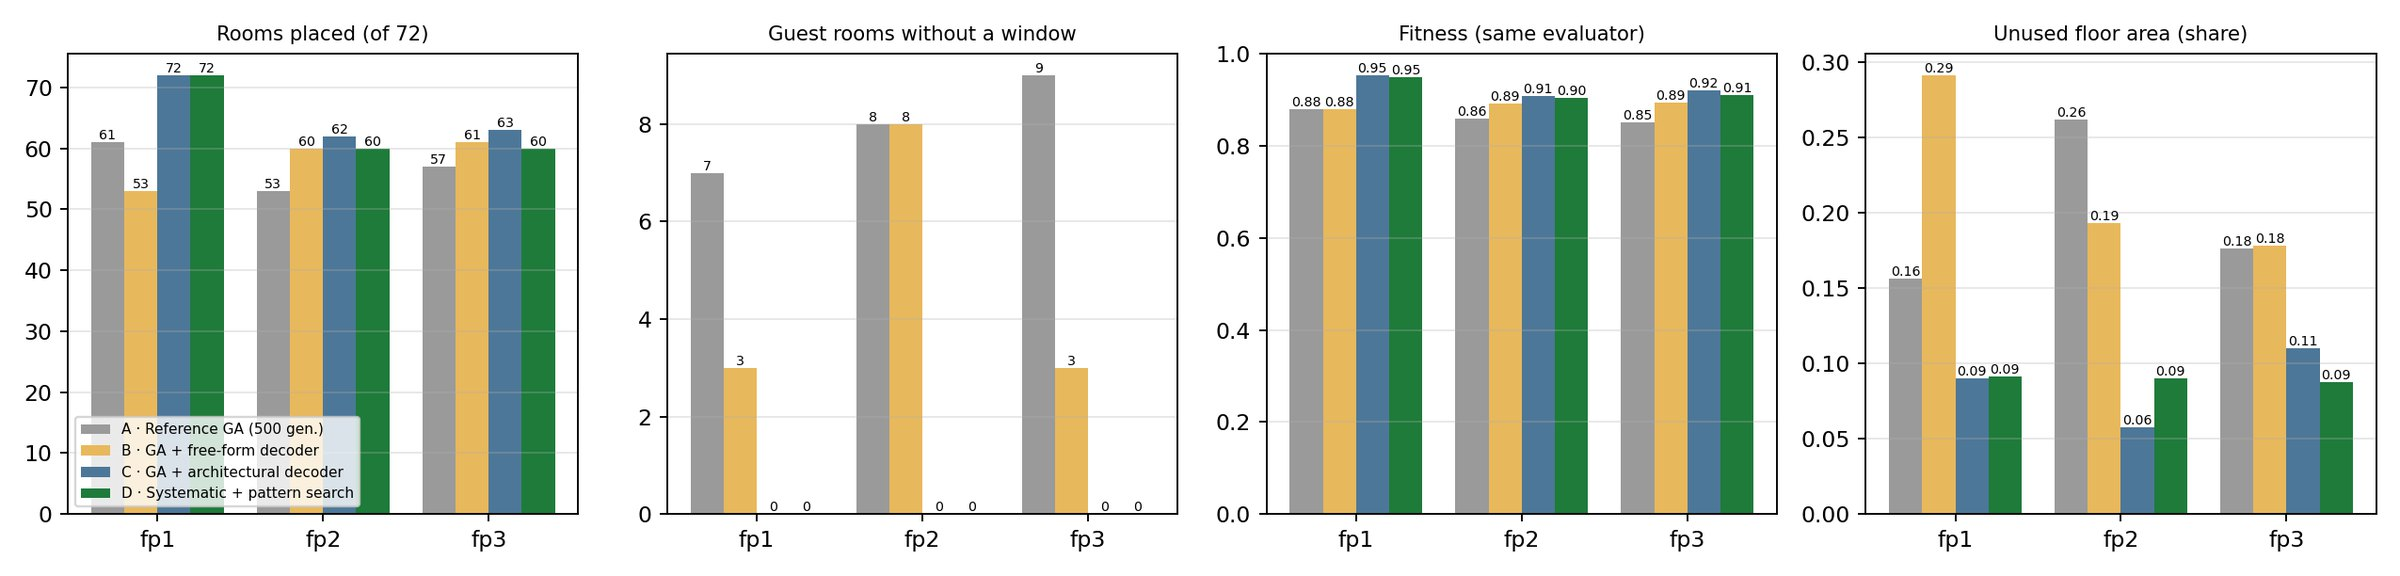
\includegraphics[width=\linewidth,keepaspectratio,height=0.30\textheight]{figures/opt_compare_bars.jpg}\caption{The four variants on the three sites (same program, same evaluator).}\end{figure}
\begin{figure}[H]\centering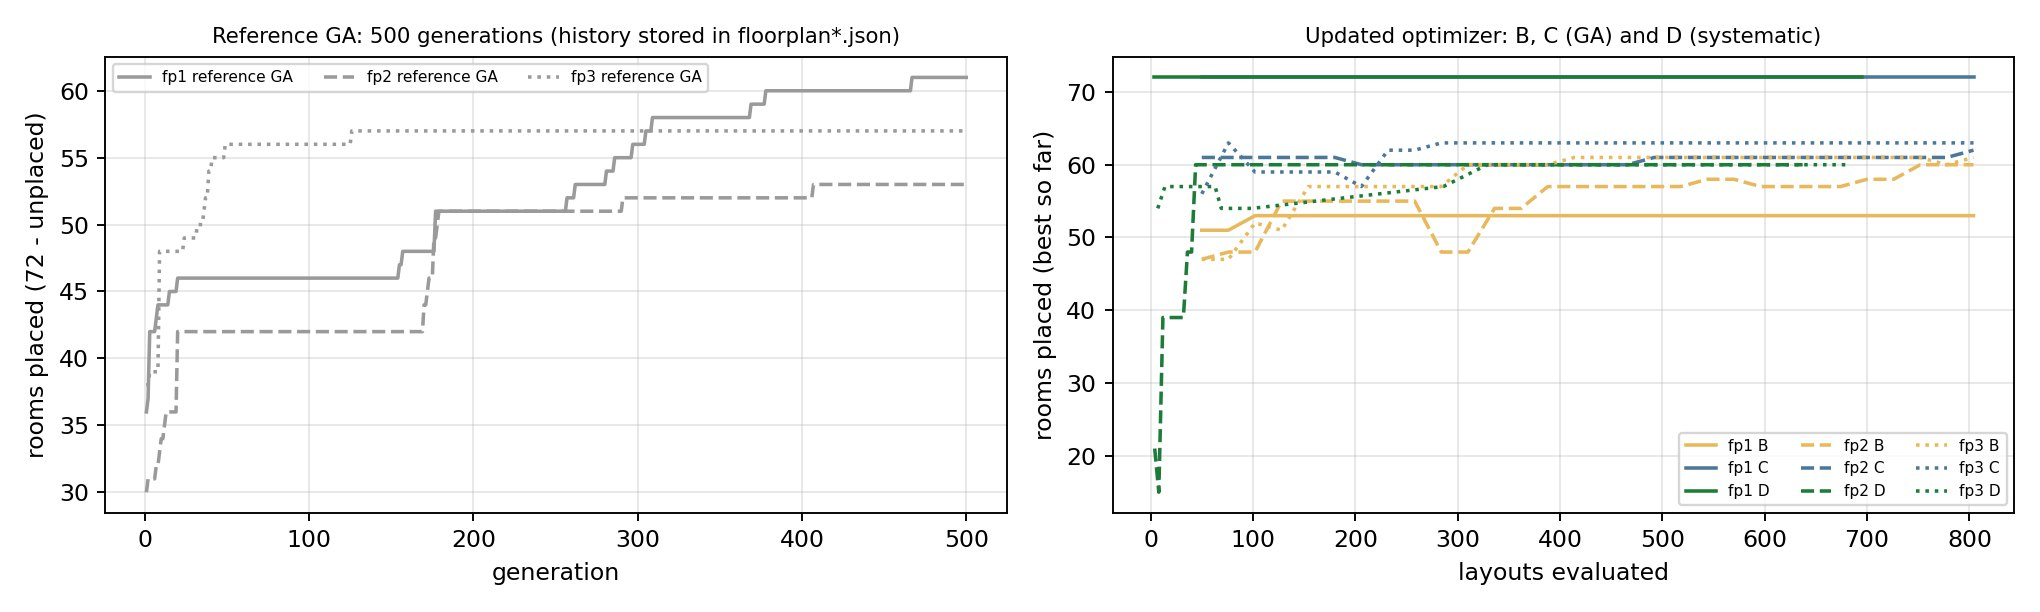
\includegraphics[width=\linewidth,keepaspectratio,height=0.30\textheight]{figures/opt_convergence.jpg}\caption{Left: rooms placed by the reference GA over its generations (from the history in the delivered files). Right: best rooms placed against layouts evaluated for the later variants.}\end{figure}
\begin{figure}[H]\centering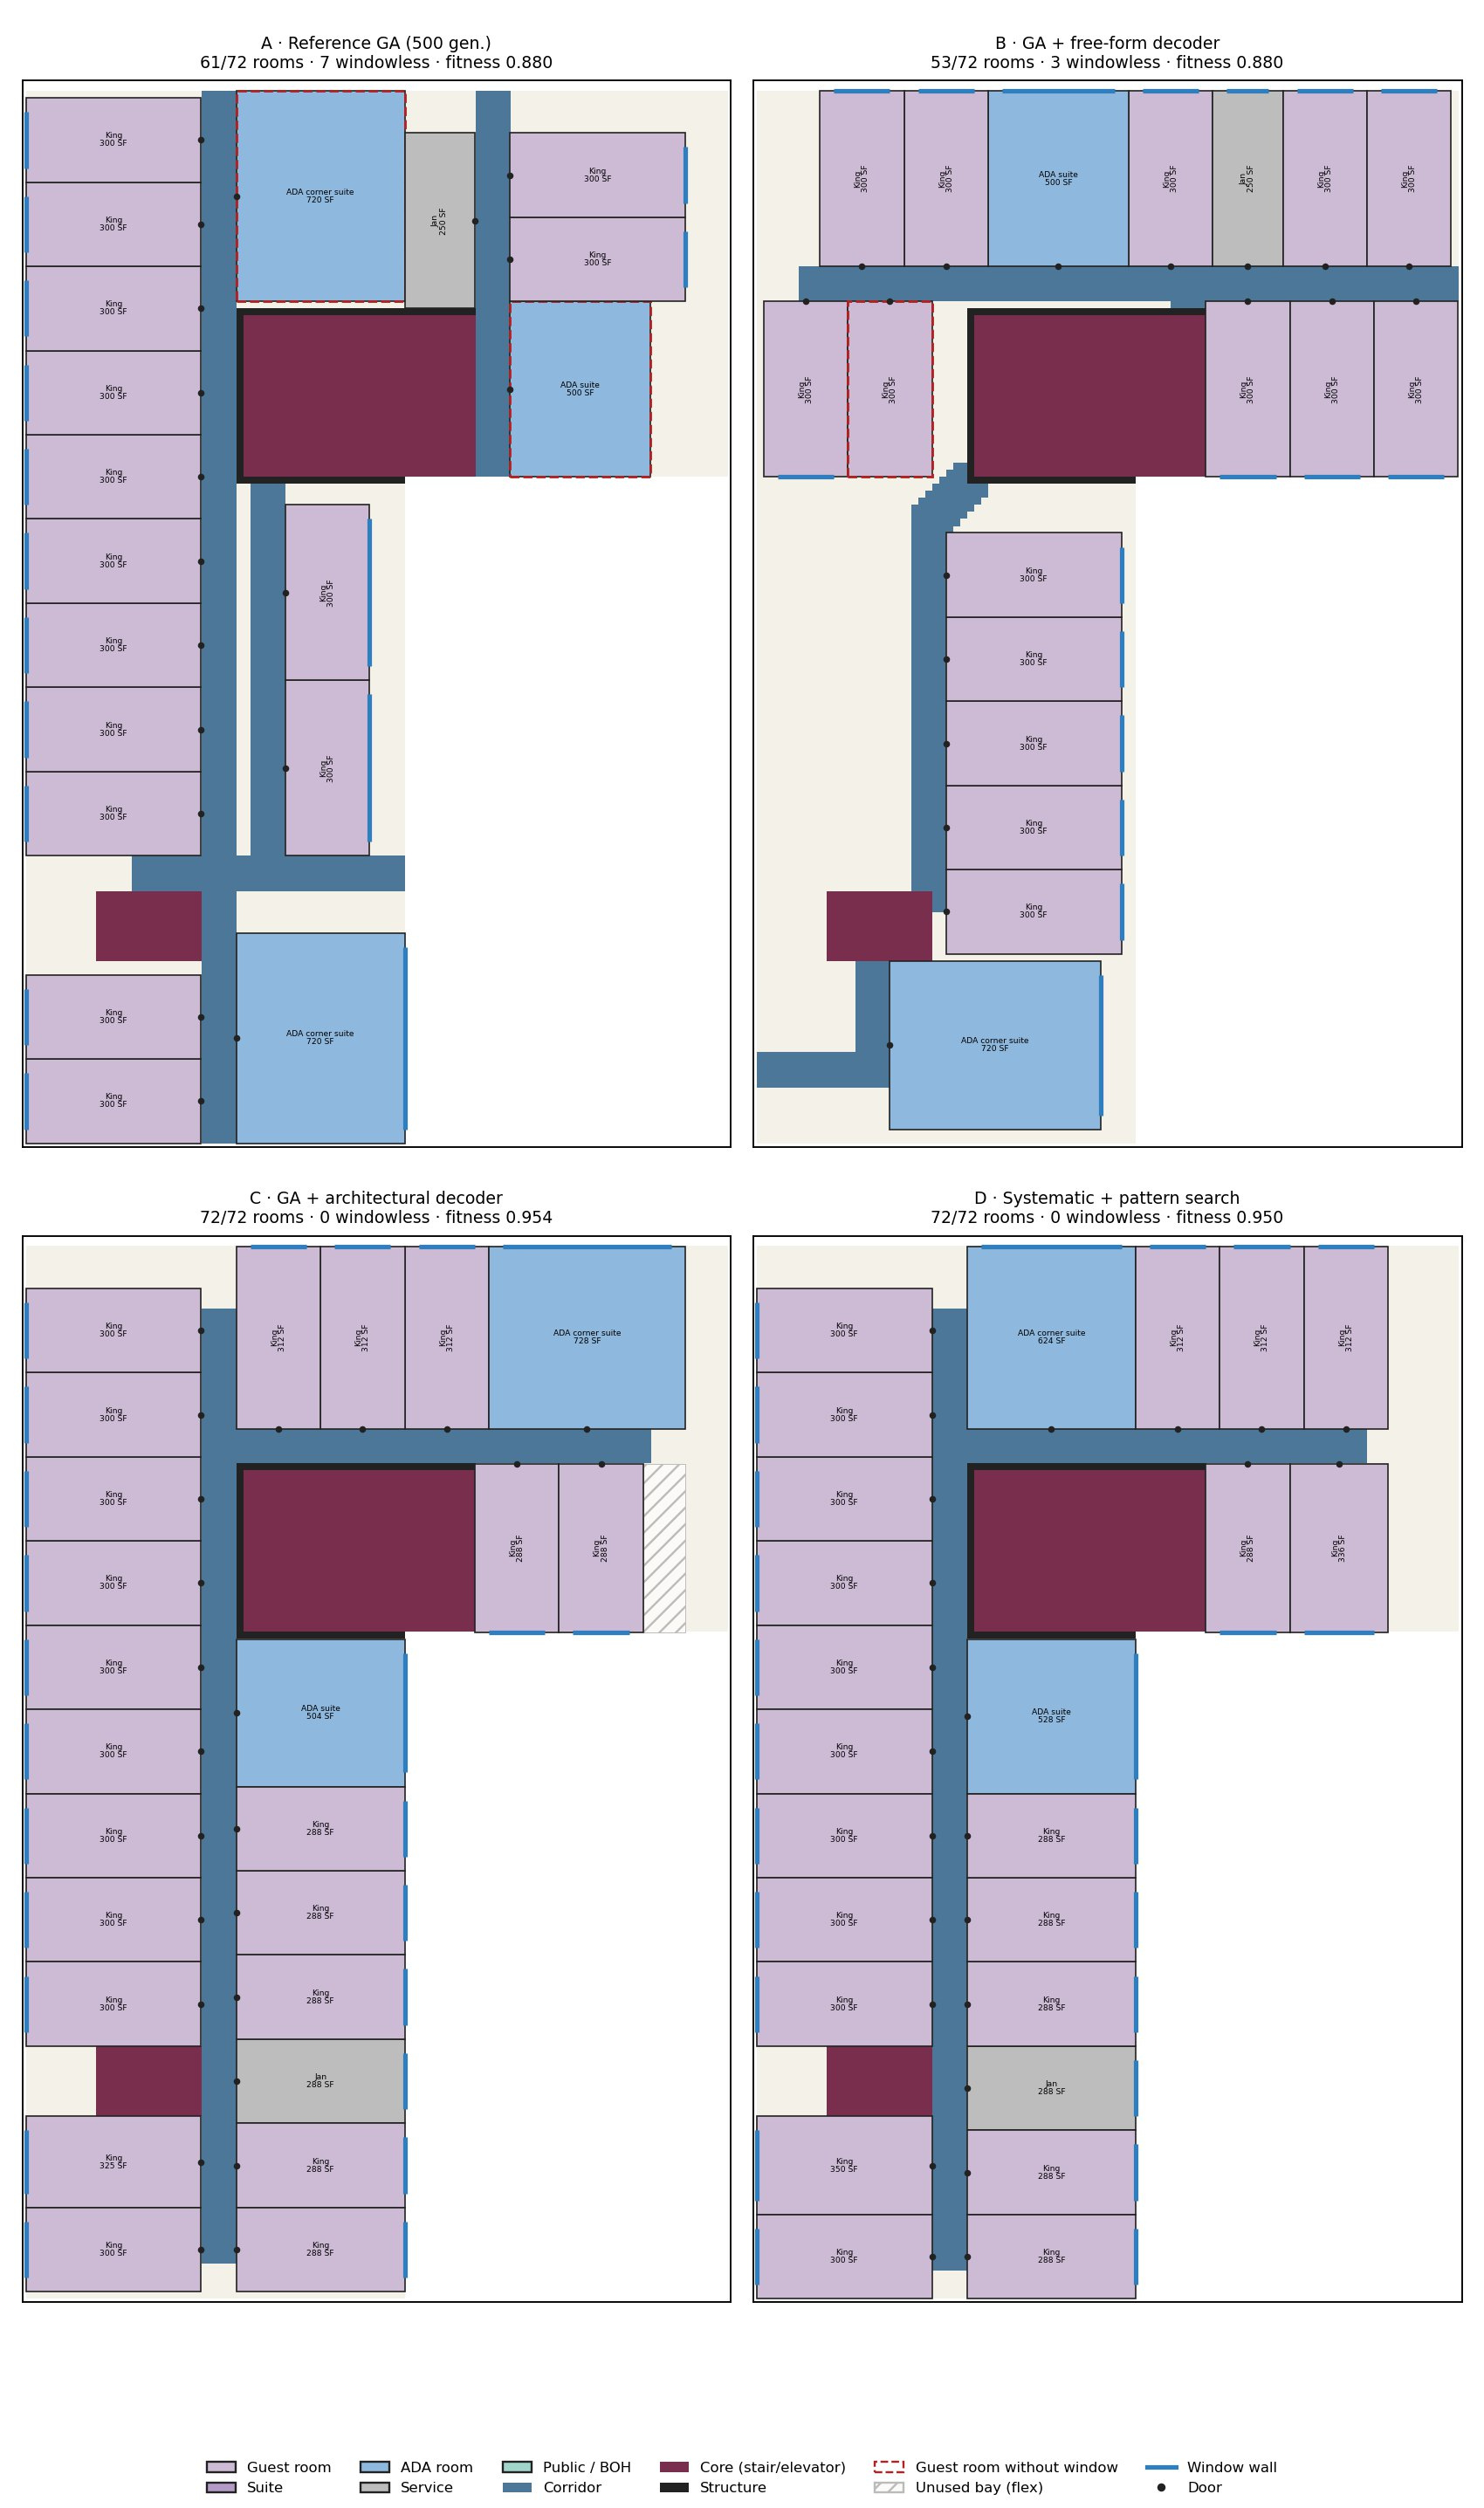
\includegraphics[width=\linewidth,keepaspectratio,height=0.80\textheight]{figures/opt_compare_fp1.jpg}\caption{Site fp1, Level 2, same program and same evaluator. Blue lines are window walls; a red dashed outline marks a guest room with no window; hatched bays are unused.}\end{figure}
\begin{figure}[H]\centering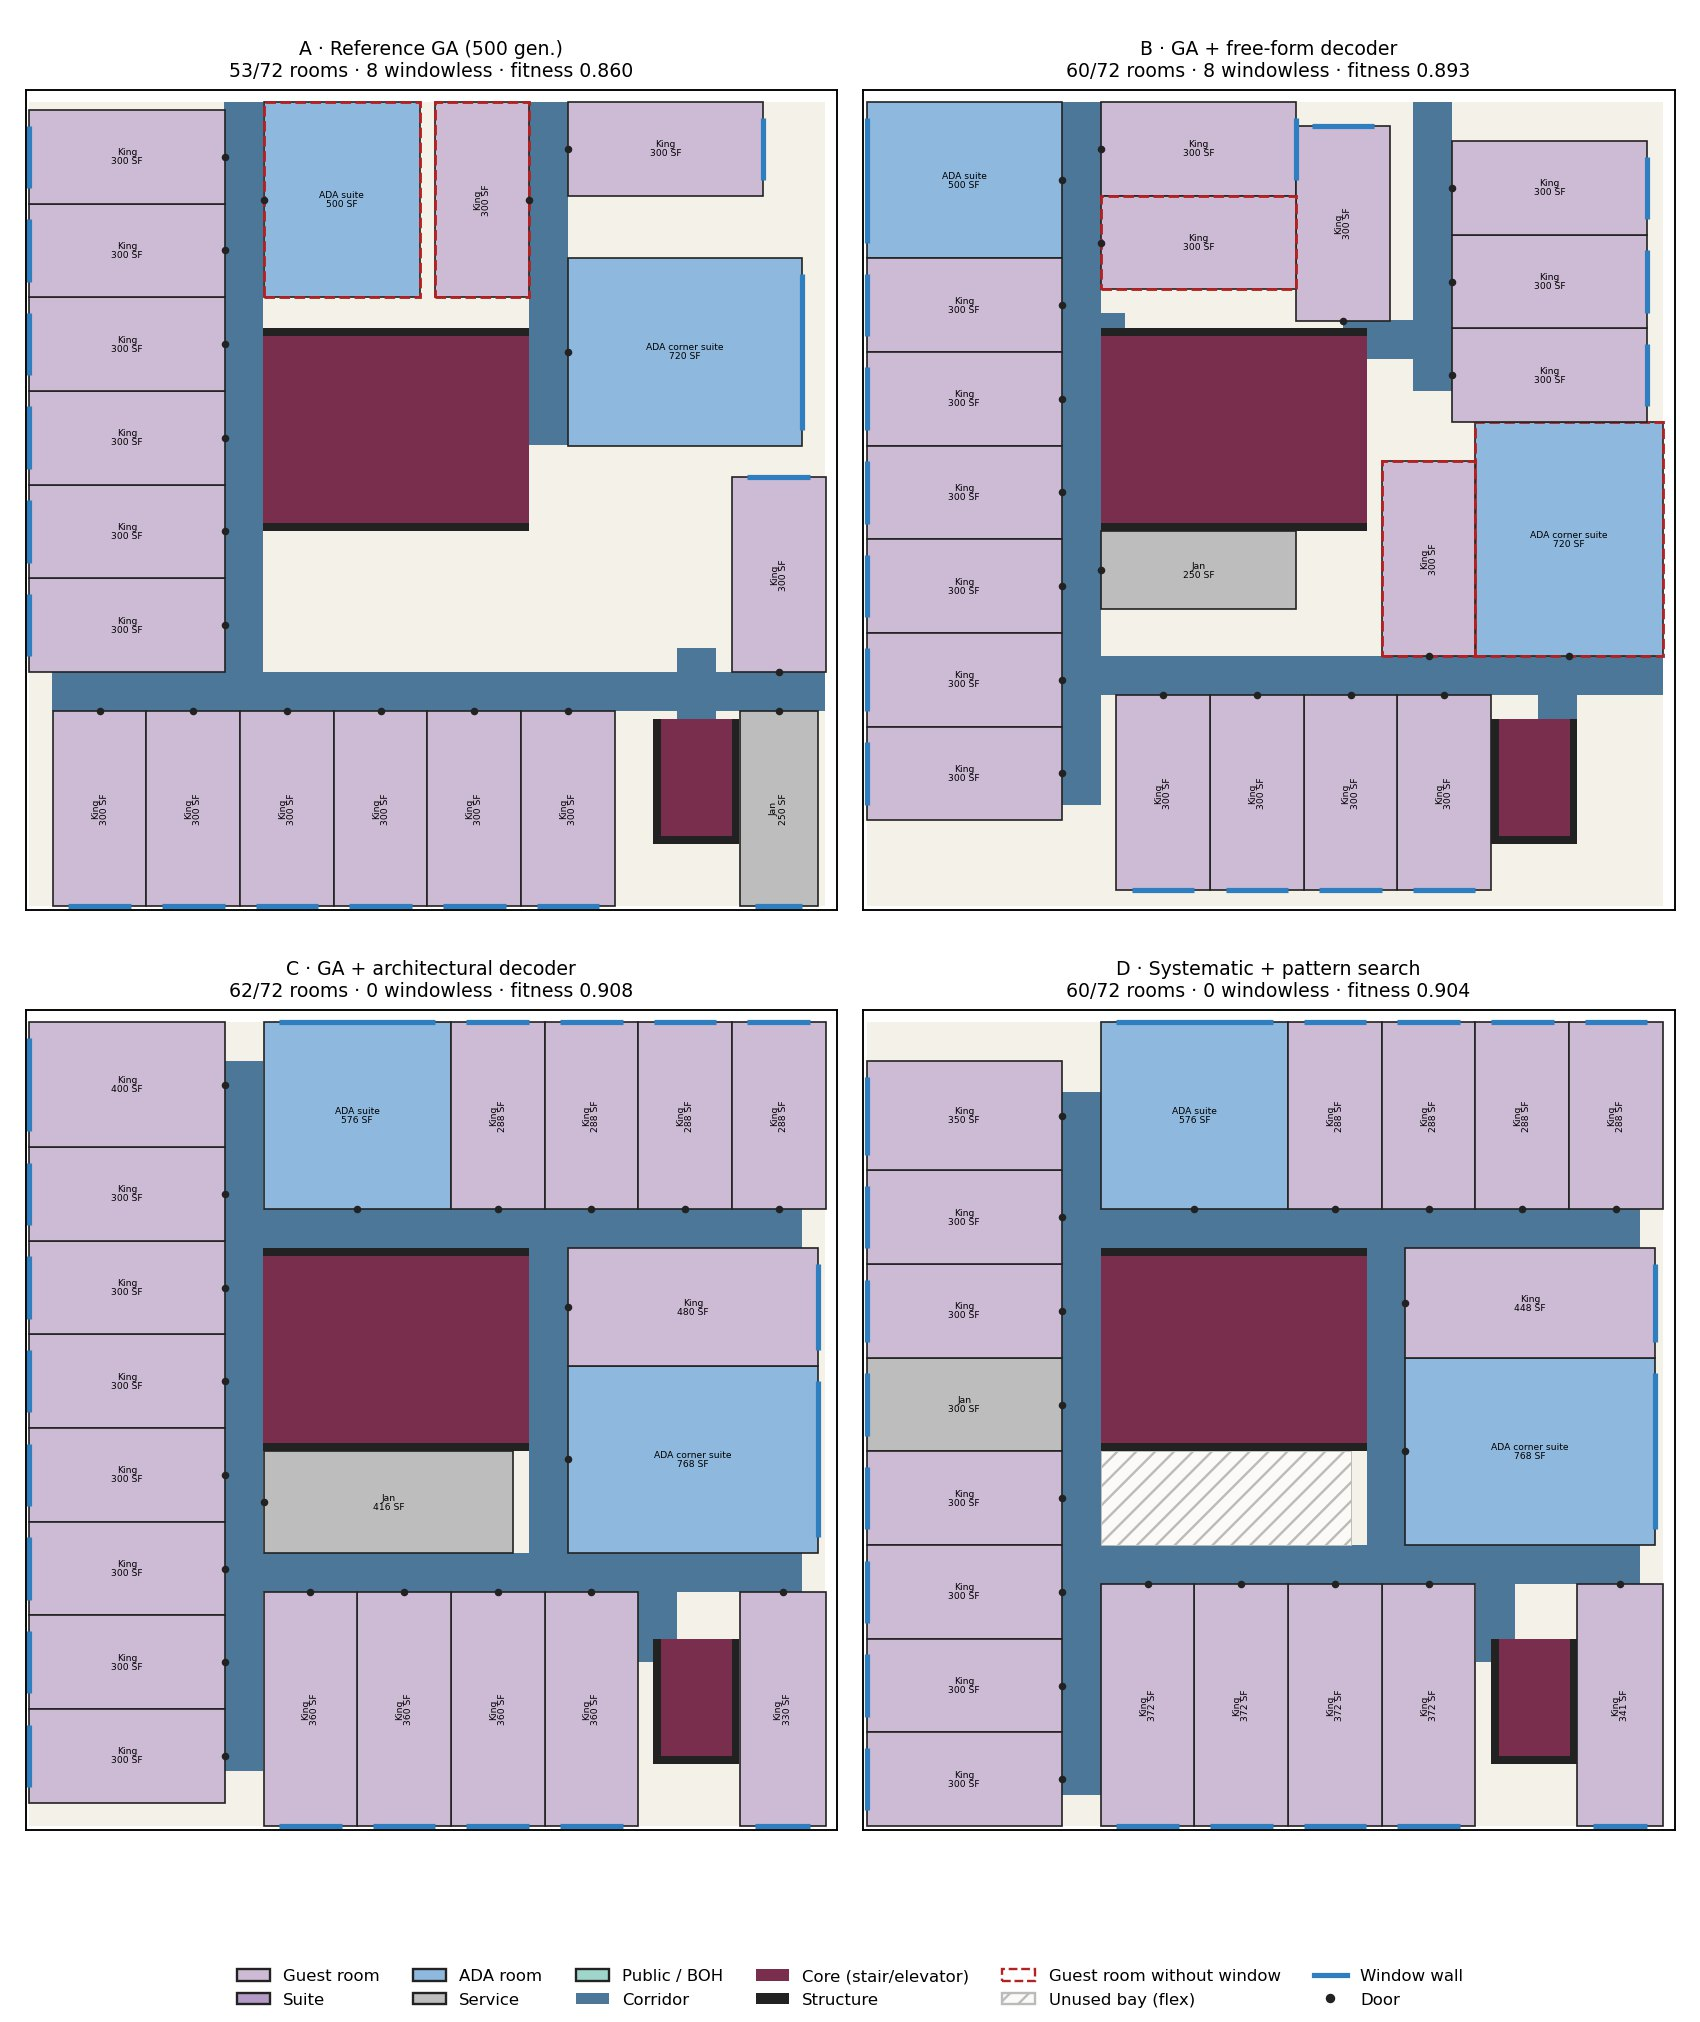
\includegraphics[width=\linewidth,keepaspectratio,height=0.80\textheight]{figures/opt_compare_fp2.jpg}\caption{Site fp2, Level 2, same program and same evaluator. Blue lines are window walls; a red dashed outline marks a guest room with no window; hatched bays are unused.}\end{figure}
\begin{figure}[H]\centering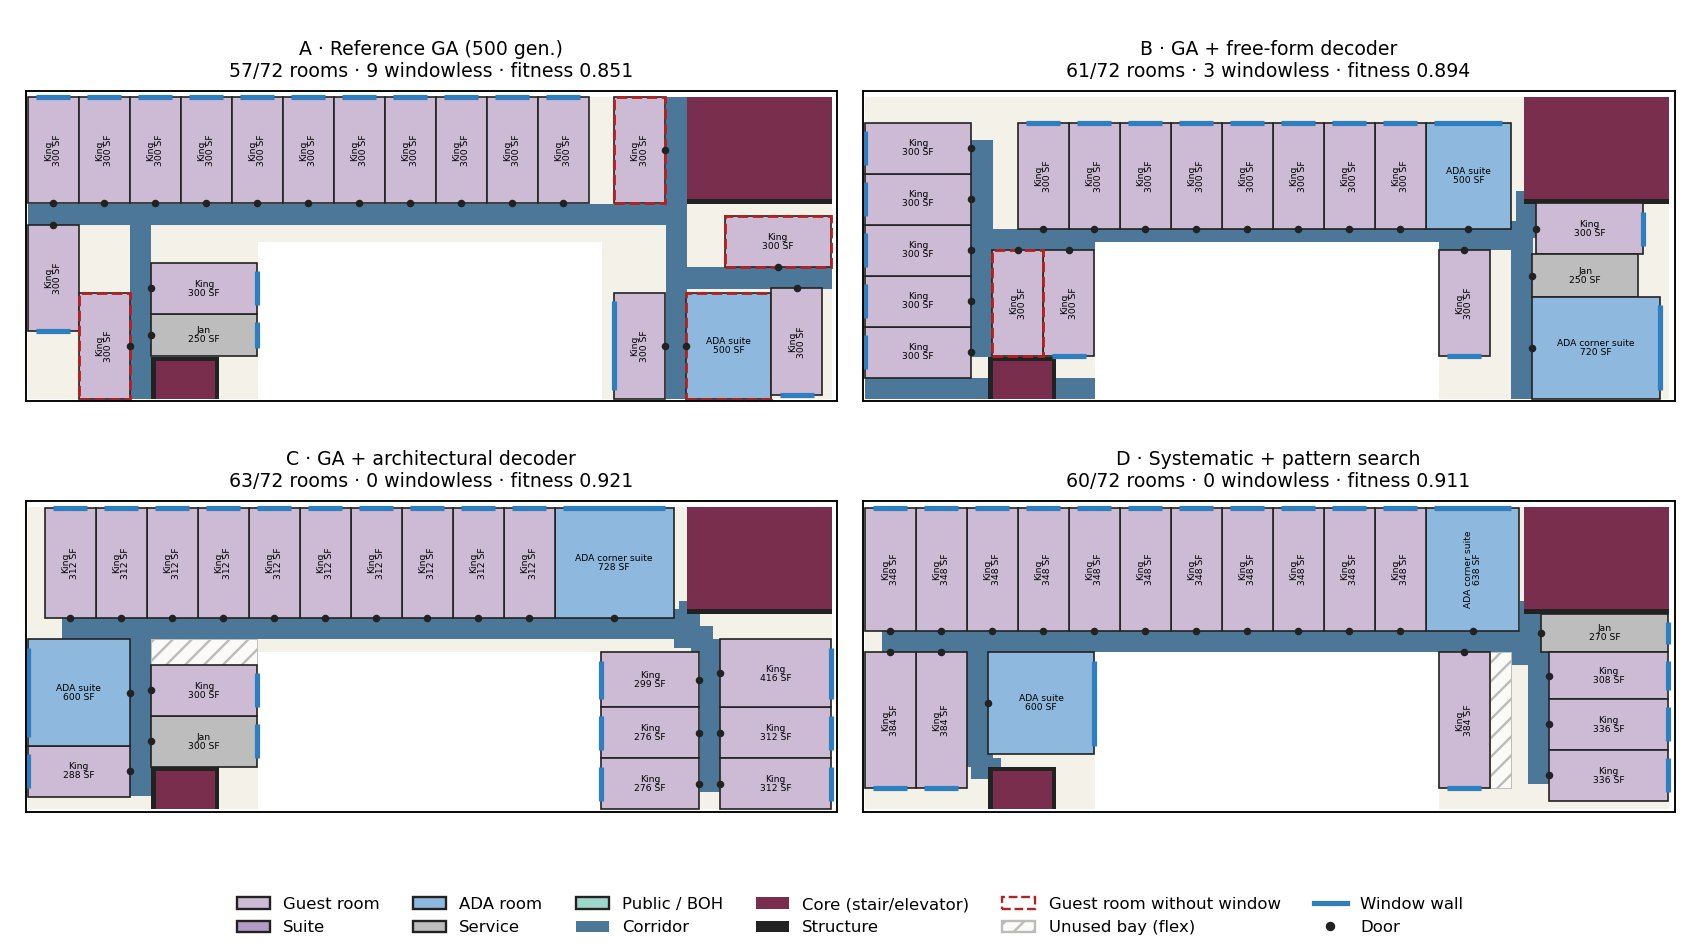
\includegraphics[width=\linewidth,keepaspectratio,height=0.80\textheight]{figures/opt_compare_fp3.jpg}\caption{Site fp3, Level 2, same program and same evaluator. Blue lines are window walls; a red dashed outline marks a guest room with no window; hatched bays are unused.}\end{figure}

\subsection{Results in Hotel Schematic (generative shape, core and floors)}\label{sec:opthotel}
Input: the Project Renegade Living + Lodging program (117 keys) and a buildable area of
170 x 265 ft. The search screened 158 plate and floor-count variants,
evaluated 1,140 layouts and kept 740 distinct ones in 36 s on eight
processes, with no LLM calls; a second run returned the same list: yes.
212 layouts are on the Pareto front. Pattern search improved the screened plates as follows:
Courtyard 156x156 $\cdot$ center core (5 fl.) 0.870 $\to$ 0.870; L 202x121 $\cdot$ ends core (5 fl.) 0.863 $\to$ 0.881; Bar 265x58 $\cdot$ center core (5 fl.) 0.863 $\to$ 0.863; T 202x121 $\cdot$ center core (5 fl.) 0.856 $\to$ 0.865.
\begingroup\captionof{table}{Top ten layouts under the Balanced decision weights.}\endgroup
{\footnotesize\begin{longtable}{p{0.38cm}p{3.99cm}p{0.95cm}p{1.14cm}p{0.85cm}p{0.76cm}p{0.95cm}p{1.04cm}p{0.85cm}p{0.85cm}p{0.95cm}p{0.76cm}}
\toprule
\textbf{\#} & \textbf{Layout} & \textbf{Guest floors} & \textbf{TOPSIS $C_j$} & \textbf{Pareto} & \textbf{Keys} & \textbf{Fitness} & \textbf{Corridor} & \textbf{SF / key} & \textbf{Height ft} & \textbf{Dead end ft} & \textbf{Code} \\ \midrule \endhead
1 & Bar 265x58 $\cdot$ center core & 4 & 0.917 & yes & 117 & 0.859 & 0.112 & 657 & 59 & 24 & 1.00 \\
2 & L 220x132 $\cdot$ knuckle core & 4 & 0.906 & yes & 117 & 0.849 & 0.120 & 729 & 59 & 26 & 1.00 \\
3 & L 170x176 $\cdot$ knuckle core & 4 & 0.905 & yes & 117 & 0.835 & 0.120 & 714 & 59 & 24 & 1.00 \\
4 & Bar 265x58 $\cdot$ ends core & 4 & 0.904 & yes & 117 & 0.845 & 0.113 & 657 & 59 & 30 & 1.00 \\
5 & Bar 265x58 $\cdot$ ends core & 4 & 0.903 & yes & 117 & 0.843 & 0.113 & 657 & 59 & 30 & 1.00 \\
6 & Bar 265x58 $\cdot$ ends core & 4 & 0.903 & yes & 117 & 0.842 & 0.113 & 657 & 59 & 31 & 1.00 \\
7 & Courtyard 156x156 $\cdot$ ends core & 4 & 0.902 & yes & 117 & 0.845 & 0.111 & 972 & 59 & 28 & 1.00 \\
8 & T 170x176 $\cdot$ knuckle core & 4 & 0.899 & no & 114 & 0.840 & 0.122 & 733 & 59 & 24 & 1.00 \\
9 & T 170x176 $\cdot$ knuckle core & 4 & 0.899 & no & 114 & 0.840 & 0.122 & 733 & 59 & 24 & 1.00 \\
10 & Bar 265x58 $\cdot$ center core & 5 & 0.897 & yes & 117 & 0.863 & 0.112 & 788 & 70 & 24 & 0.86 \\
\bottomrule
\end{longtable}}\addtocounter{table}{-1}
\begingroup\captionof{table}{Best layout of each shape (Balanced weights).}\endgroup
{\footnotesize\begin{longtable}{p{1.61cm}p{4.37cm}p{1.04cm}p{1.14cm}p{0.85cm}p{1.04cm}p{1.33cm}p{1.14cm}p{0.85cm}}
\toprule
\textbf{Shape} & \textbf{Best layout of that shape} & \textbf{Guest floors} & \textbf{Overall rank} & \textbf{Keys} & \textbf{SF / key} & \textbf{Facade ft / key} & \textbf{Dead end ft} & \textbf{Code} \\ \midrule \endhead
Bar & Bar 265x58 $\cdot$ center core & 4 & 1 & 117 & 657 & 27.6 & 24 & 1.00 \\
L & L 220x132 $\cdot$ knuckle core & 4 & 2 & 117 & 729 & 30.1 & 26 & 1.00 \\
Courtyard & Courtyard 156x156 $\cdot$ ends core & 4 & 7 & 117 & 972 & 33.5 & 28 & 1.00 \\
T & T 170x176 $\cdot$ knuckle core & 4 & 8 & 114 & 733 & 30.4 & 24 & 1.00 \\
U & U 187x112 $\cdot$ center core & 4 & 34 & 111 & 771 & 31.8 & 29 & 1.00 \\
H & H 156x136 $\cdot$ knuckle core & 4 & 206 & 106 & 854 & 34.9 & 59 & 0.86 \\
\bottomrule
\end{longtable}}\addtocounter{table}{-1}
\begingroup\captionof{table}{The first-ranked layout changes with the decision priority: the trade-off is the user's, the search only supplies the options.}\endgroup
{\footnotesize\begin{longtable}{p{2.66cm}p{4.94cm}p{1.23cm}p{0.95cm}p{1.14cm}p{1.23cm}p{0.95cm}}
\toprule
\textbf{Decision priority} & \textbf{Layout ranked first} & \textbf{Guest floors} & \textbf{Keys} & \textbf{SF / key} & \textbf{Height ft} & \textbf{Code} \\ \midrule \endhead
Balanced & Bar 265x58 $\cdot$ center core & 4 & 117 & 657 & 59 & 1.00 \\
Most keys & Courtyard 156x156 $\cdot$ center core & 4 & 117 & 972 & 59 & 1.00 \\
Lowest cost & Bar 265x58 $\cdot$ center core & 4 & 117 & 657 & 59 & 1.00 \\
Guest experience & Bar 265x58 $\cdot$ center core & 4 & 117 & 657 & 59 & 1.00 \\
Low-rise & Bar 265x58 $\cdot$ center core & 4 & 117 & 657 & 59 & 1.00 \\
\bottomrule
\end{longtable}}\addtocounter{table}{-1}
\textbf{First-ranked layout: Bar 265x58 $\cdot$ center core, 4 guest floors.} Footprint 265 x 58 ft
(15,370 SF), 2 elevators, bay module 13 ft. It places
117 of 117 keys and 142 of 150 program rooms; the
frontage bound is 34 keys per typical floor. Corridor share 0.112, longest exit
travel 64 ft, dead end 24 ft, fitness 0.859. Not placed: White Box Retail x1, IT x1, Jan x2, Gym x1, MEP Service x1, Loading x1, Luggage x1.
{\footnotesize\begin{longtable}{p{1.80cm}p{4.37cm}p{4.37cm}p{2.28cm}p{1.23cm}}
\toprule
\textbf{Rule} & \textbf{Check} & \textbf{Required} & \textbf{Provided} & \textbf{Status} \\ \midrule \endhead
IBC-R1-015 & Exits per story (cores reached) & $\ge$ 2 & 3 & \textcolor{pass}{\textbf{PASS}} \\
IBC-R1-018 & Exit separation (core to core) & $\ge$ 1/3 diagonal = 90 ft & 202 ft & \textcolor{pass}{\textbf{PASS}} \\
IBC-R1-023 & Exit access travel & $\le$ 250 ft & 63 ft & \textcolor{pass}{\textbf{PASS}} \\
IBC-R1-025 & Corridor width & $\ge$ 44 in & 72 in & \textcolor{pass}{\textbf{PASS}} \\
IBC-R1-027 & Dead-end corridor & $\le$ 50 ft & 24 ft & \textcolor{pass}{\textbf{PASS}} \\
ADA-224.2 & ADA mobility rooms & $\ge$ 7 for 117 keys & 7 & \textcolor{pass}{\textbf{PASS}} \\
IBC-R1-007 & Stories above grade & $\le$ 5 (Type IIA, sprinklered R-1) & 5 & \textcolor{pass}{\textbf{PASS}} \\
\bottomrule
\end{longtable}}\addtocounter{table}{-1}
\begin{figure}[H]\centering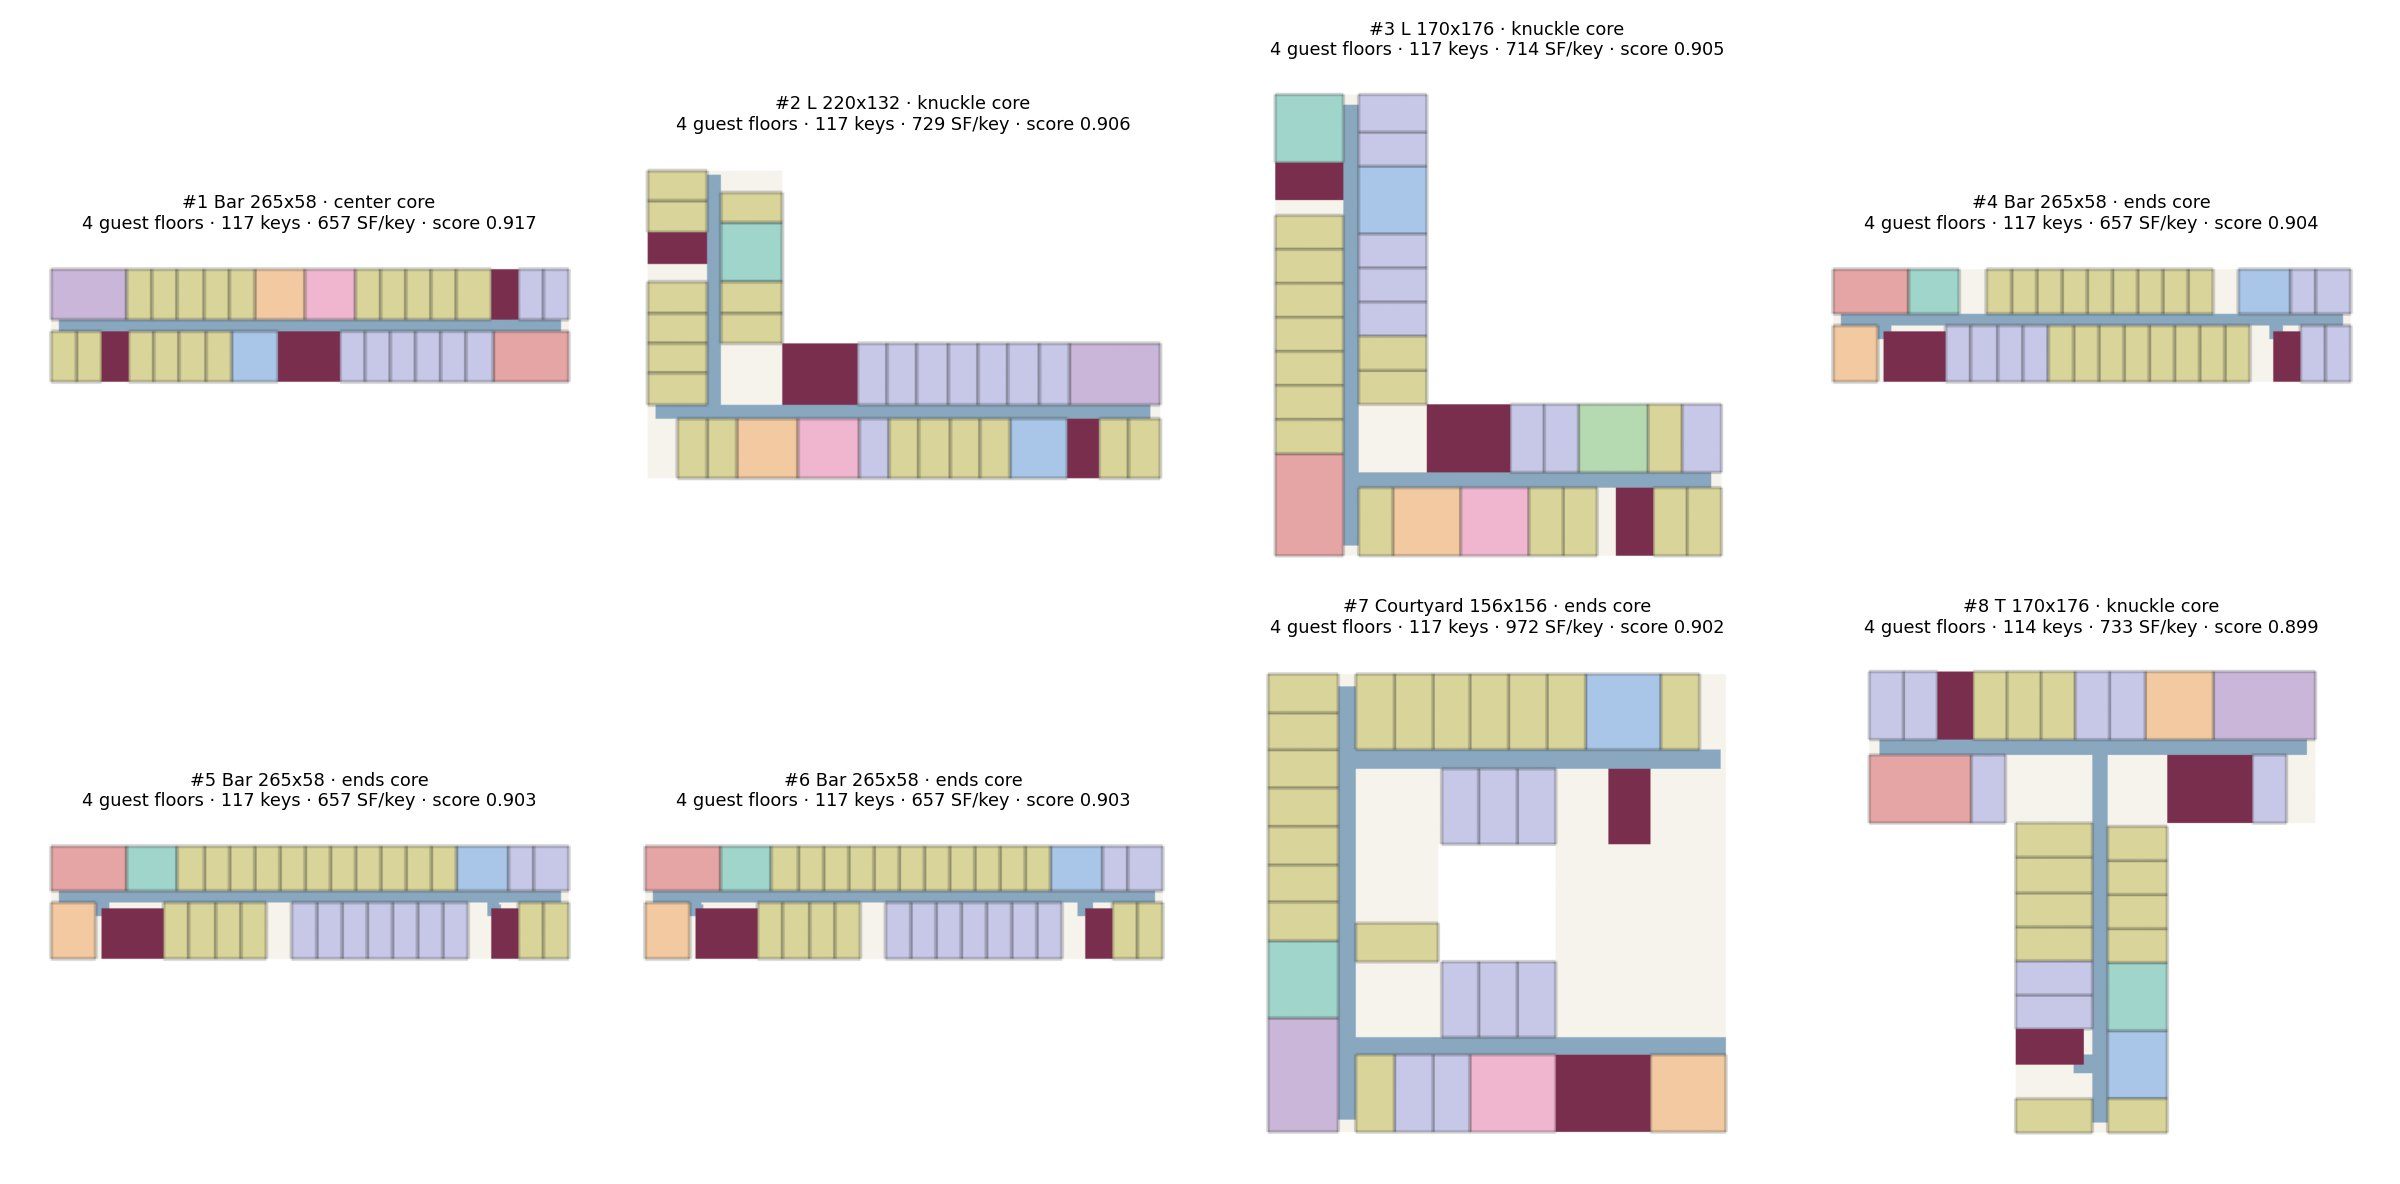
\includegraphics[width=\linewidth,keepaspectratio,height=0.45\textheight]{figures/opt_hotel_gallery.jpg}\caption{The eight first-ranked layouts (typical guest floor). Dark red: core and stairs; blue: corridor.}\end{figure}
\begin{figure}[H]\centering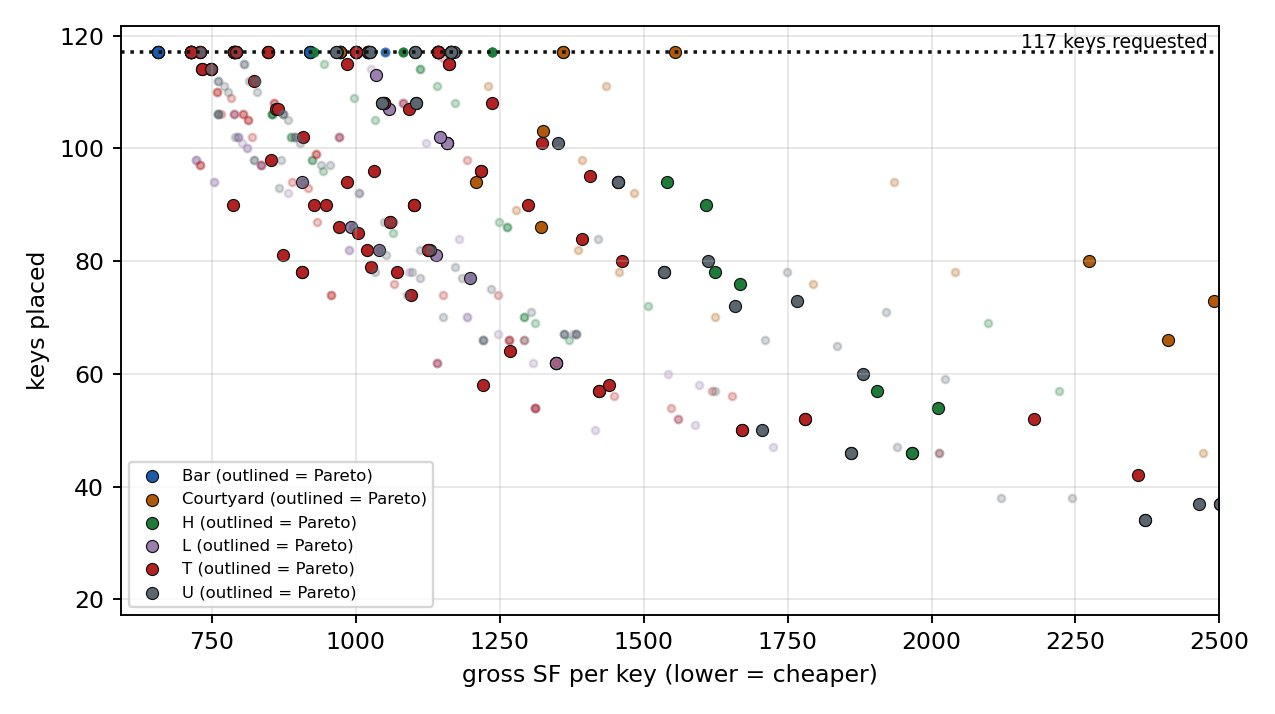
\includegraphics[width=\linewidth,keepaspectratio,height=0.34\textheight]{figures/opt_hotel_pareto.jpg}\caption{Every layout found: keys placed against gross area per key. Outlined points are on the Pareto front.}\end{figure}
\begin{figure}[H]\centering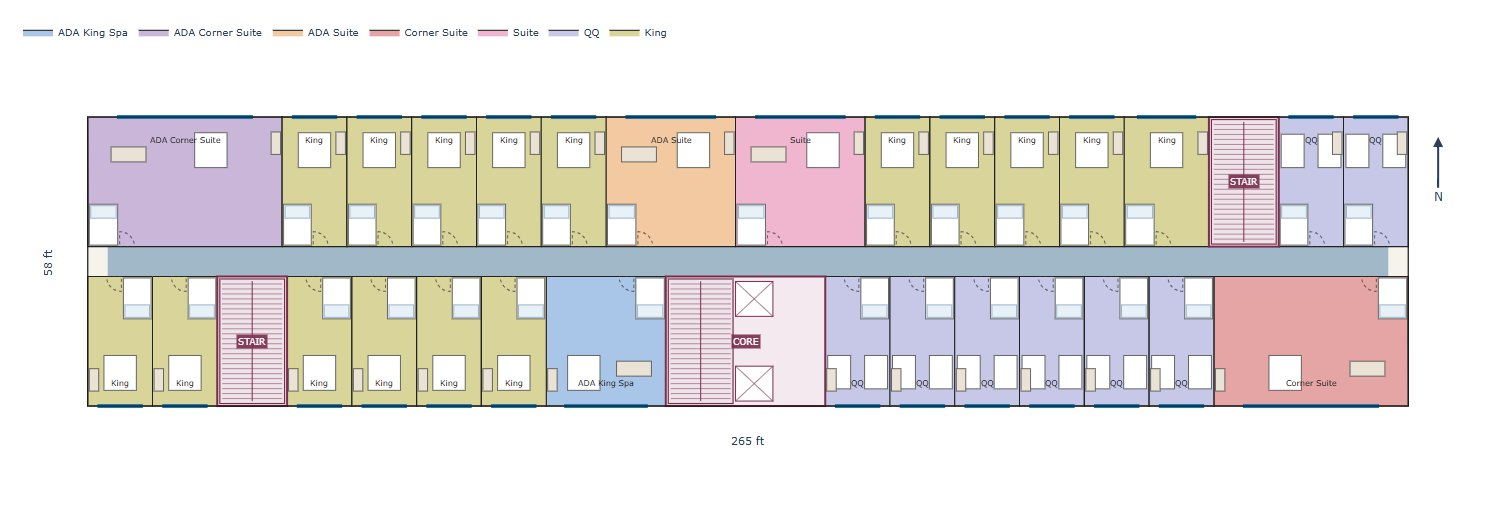
\includegraphics[width=\linewidth,keepaspectratio,height=0.40\textheight]{figures/opt_hotel_best_L2.jpg}\caption{First-ranked layout, Level 2, as drawn in the app: furnished rooms, door swings, windows (blue), stairs and elevators.}\end{figure}
\begin{figure}[H]\centering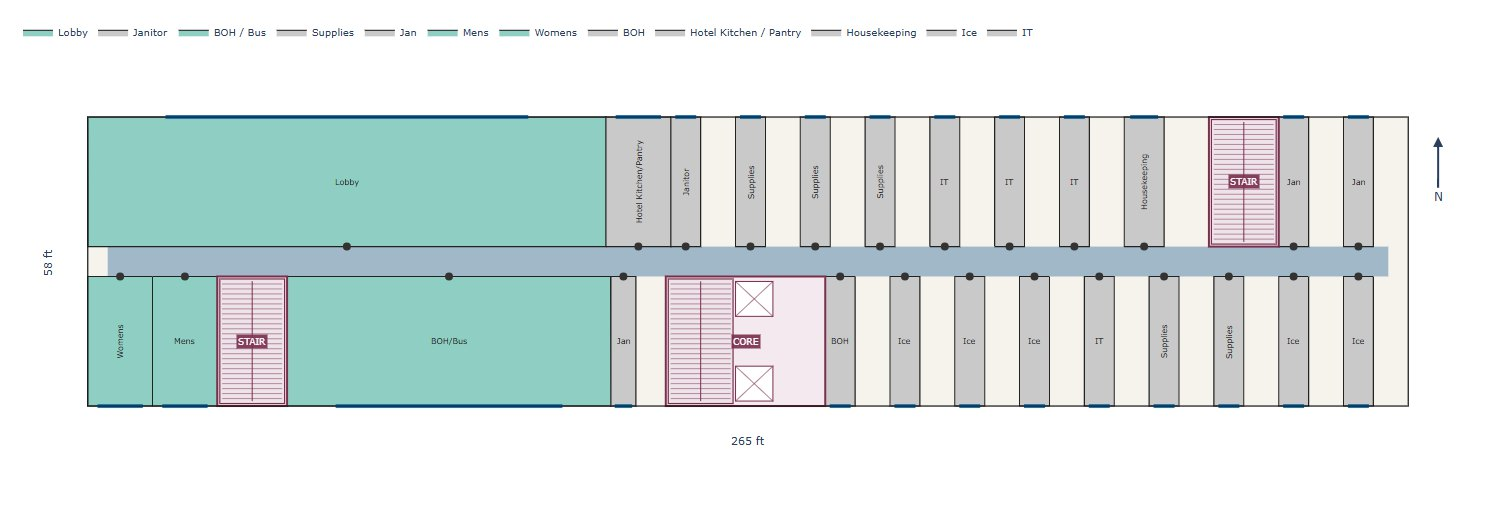
\includegraphics[width=\linewidth,keepaspectratio,height=0.40\textheight]{figures/opt_hotel_best_L1.jpg}\caption{First-ranked layout, Level 1 (public and back-of-house rooms).}\end{figure}
\begin{figure}[H]\centering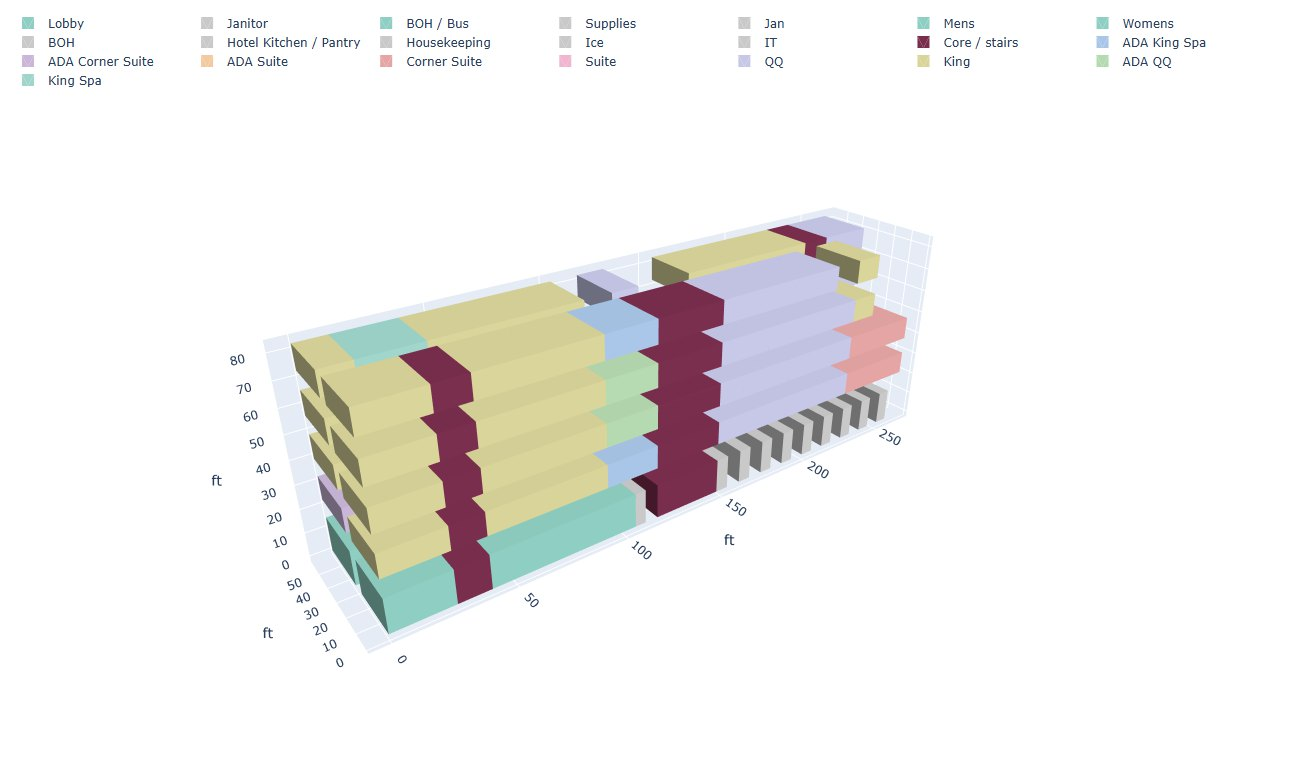
\includegraphics[width=\linewidth,keepaspectratio,height=0.38\textheight]{figures/opt_hotel_best_3d.jpg}\caption{First-ranked layout, stacked massing with the floors pulled apart.}\end{figure}

\subsection{App screenshots}
\begin{figure}[H]\centering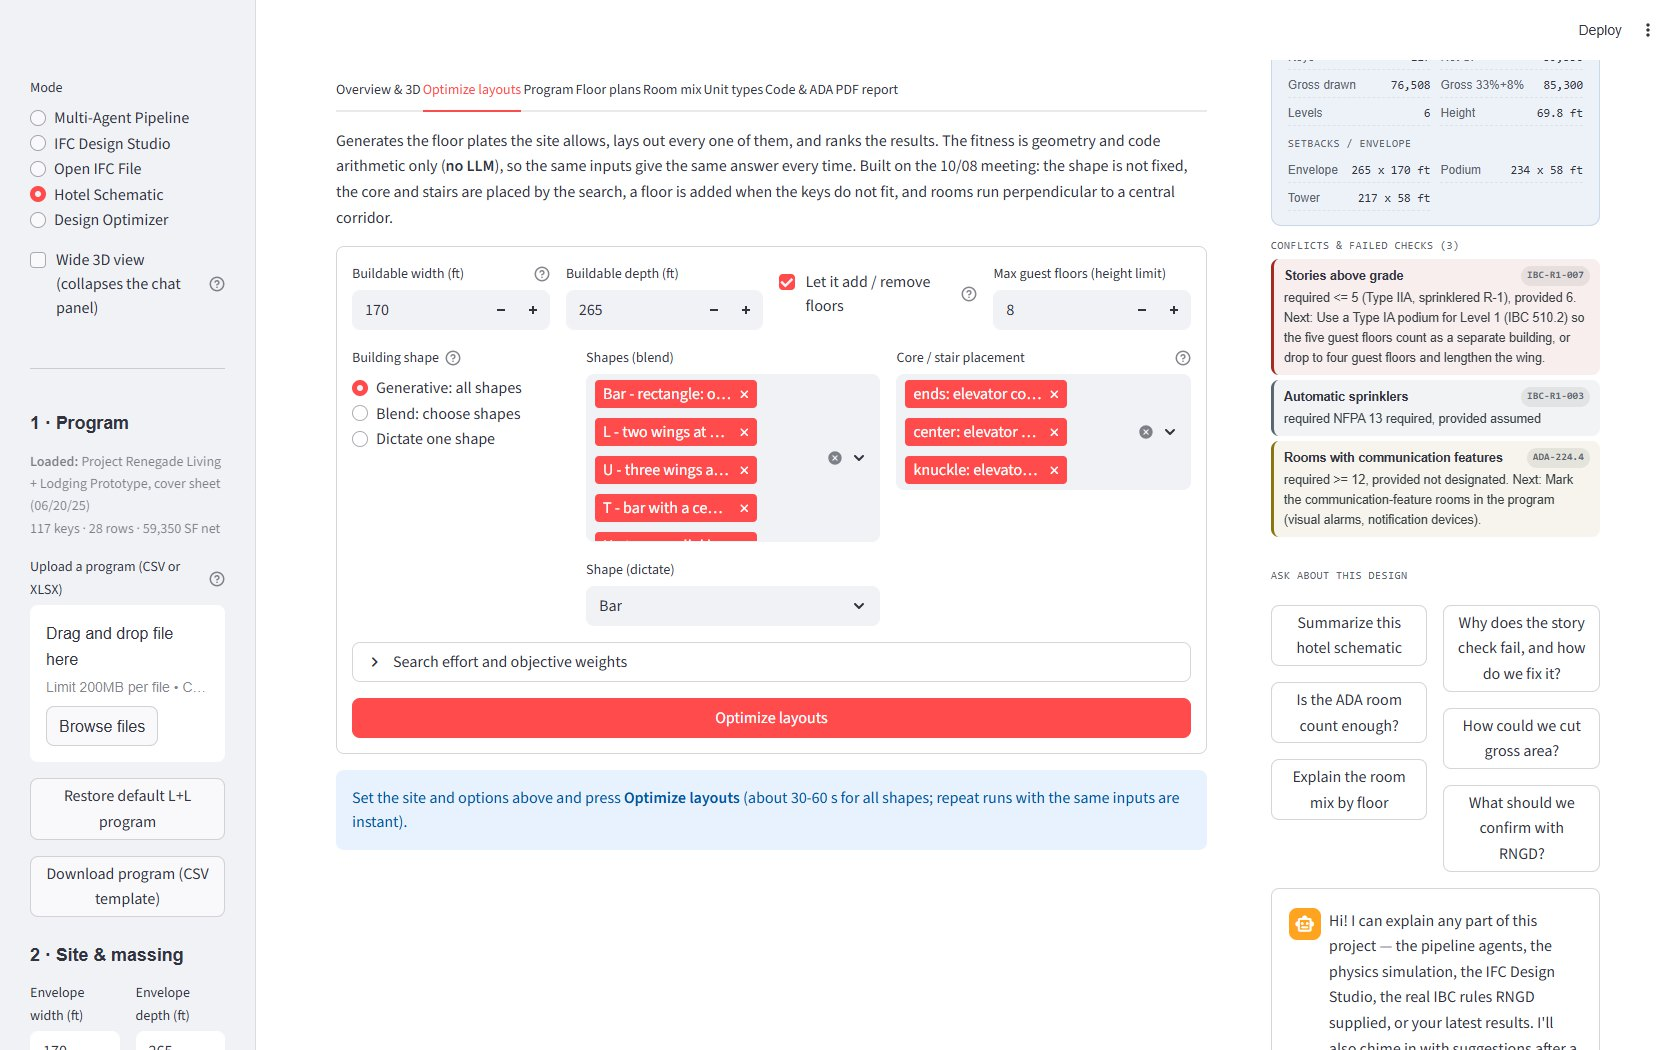
\includegraphics[width=\linewidth,keepaspectratio,height=0.42\textheight]{figures/snap_32_hotel_optimize_settings.jpg}\caption{Optimize layouts: buildable area, shape mode (generative, blend or one shape), core placement and floors.}\end{figure}
\begin{figure}[H]\centering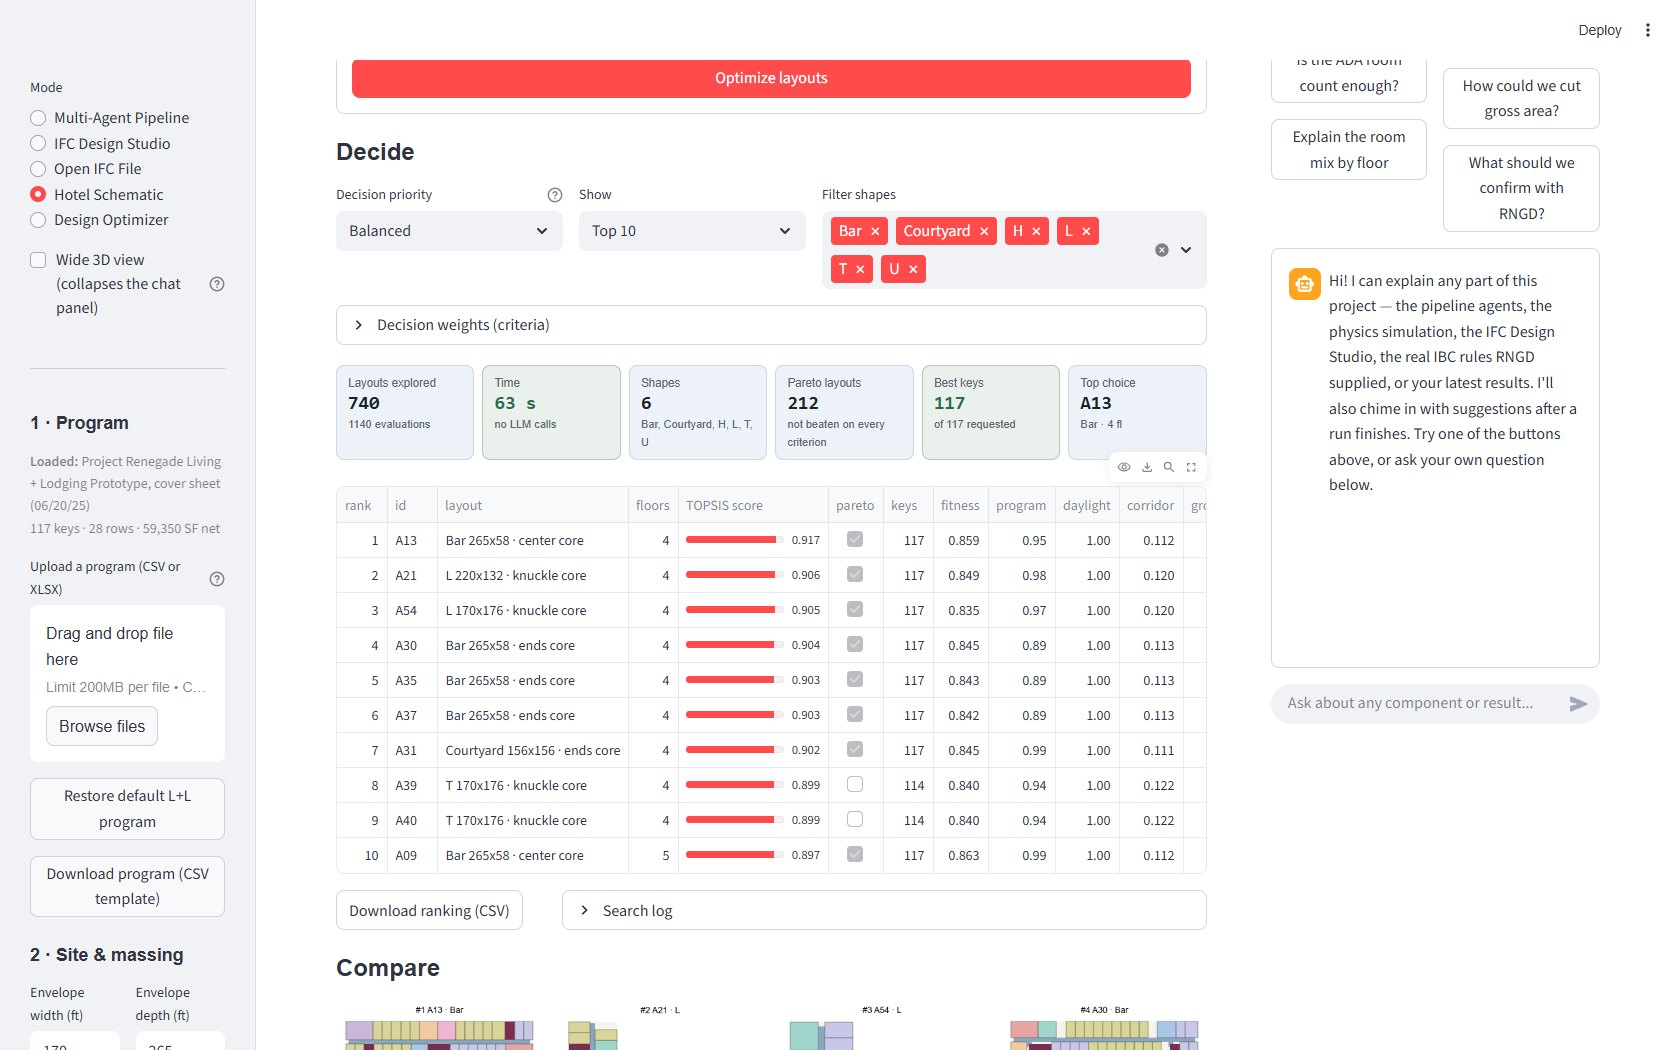
\includegraphics[width=\linewidth,keepaspectratio,height=0.42\textheight]{figures/snap_33_hotel_optimize_decide.jpg}\caption{Decision step: every distinct layout ranked by TOPSIS under the chosen priority, with the Pareto flag; the Show dropdown switches between the top 5, 10 or 25, the Pareto front and all layouts.}\end{figure}
\begin{figure}[H]\centering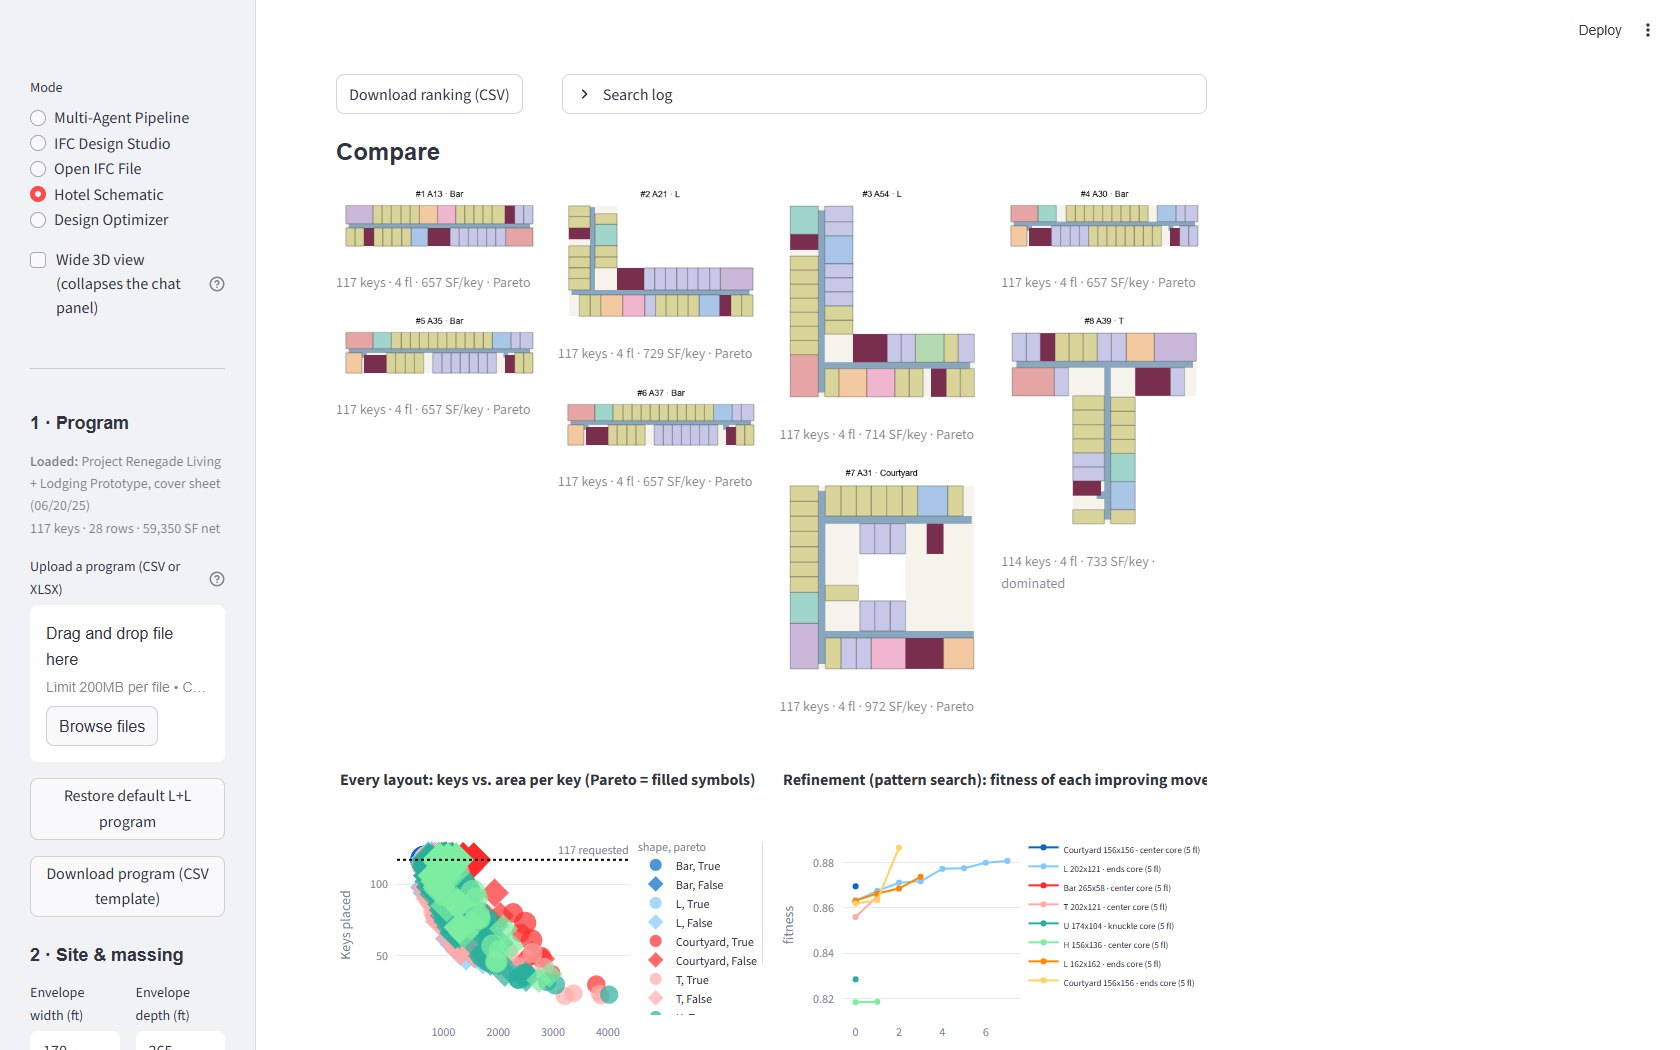
\includegraphics[width=\linewidth,keepaspectratio,height=0.42\textheight]{figures/snap_34_hotel_optimize_compare.jpg}\caption{Comparison: typical-floor thumbnails of the first-ranked layouts, keys against gross area per key for every layout, and the fitness gained by pattern search.}\end{figure}
\begin{figure}[H]\centering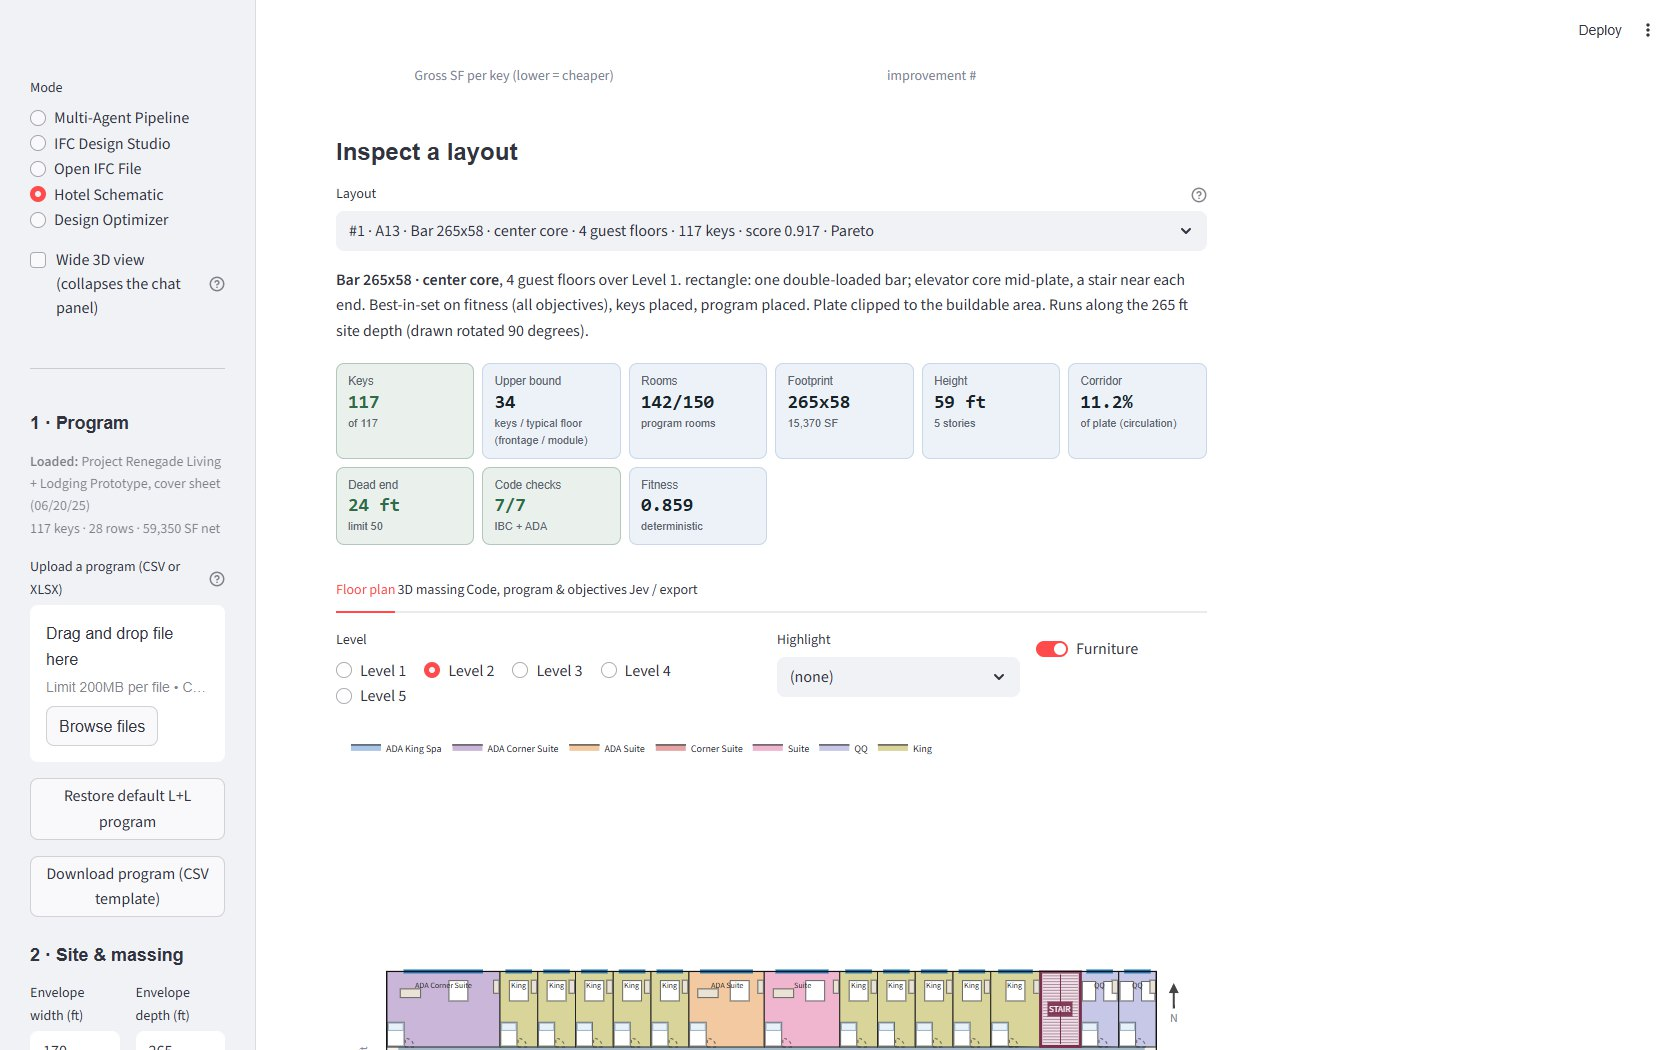
\includegraphics[width=\linewidth,keepaspectratio,height=0.42\textheight]{figures/snap_35_hotel_optimize_inspect.jpg}\caption{One layout inspected: keys, upper bound, footprint, corridor share, dead end, code checks and fitness.}\end{figure}
\begin{figure}[H]\centering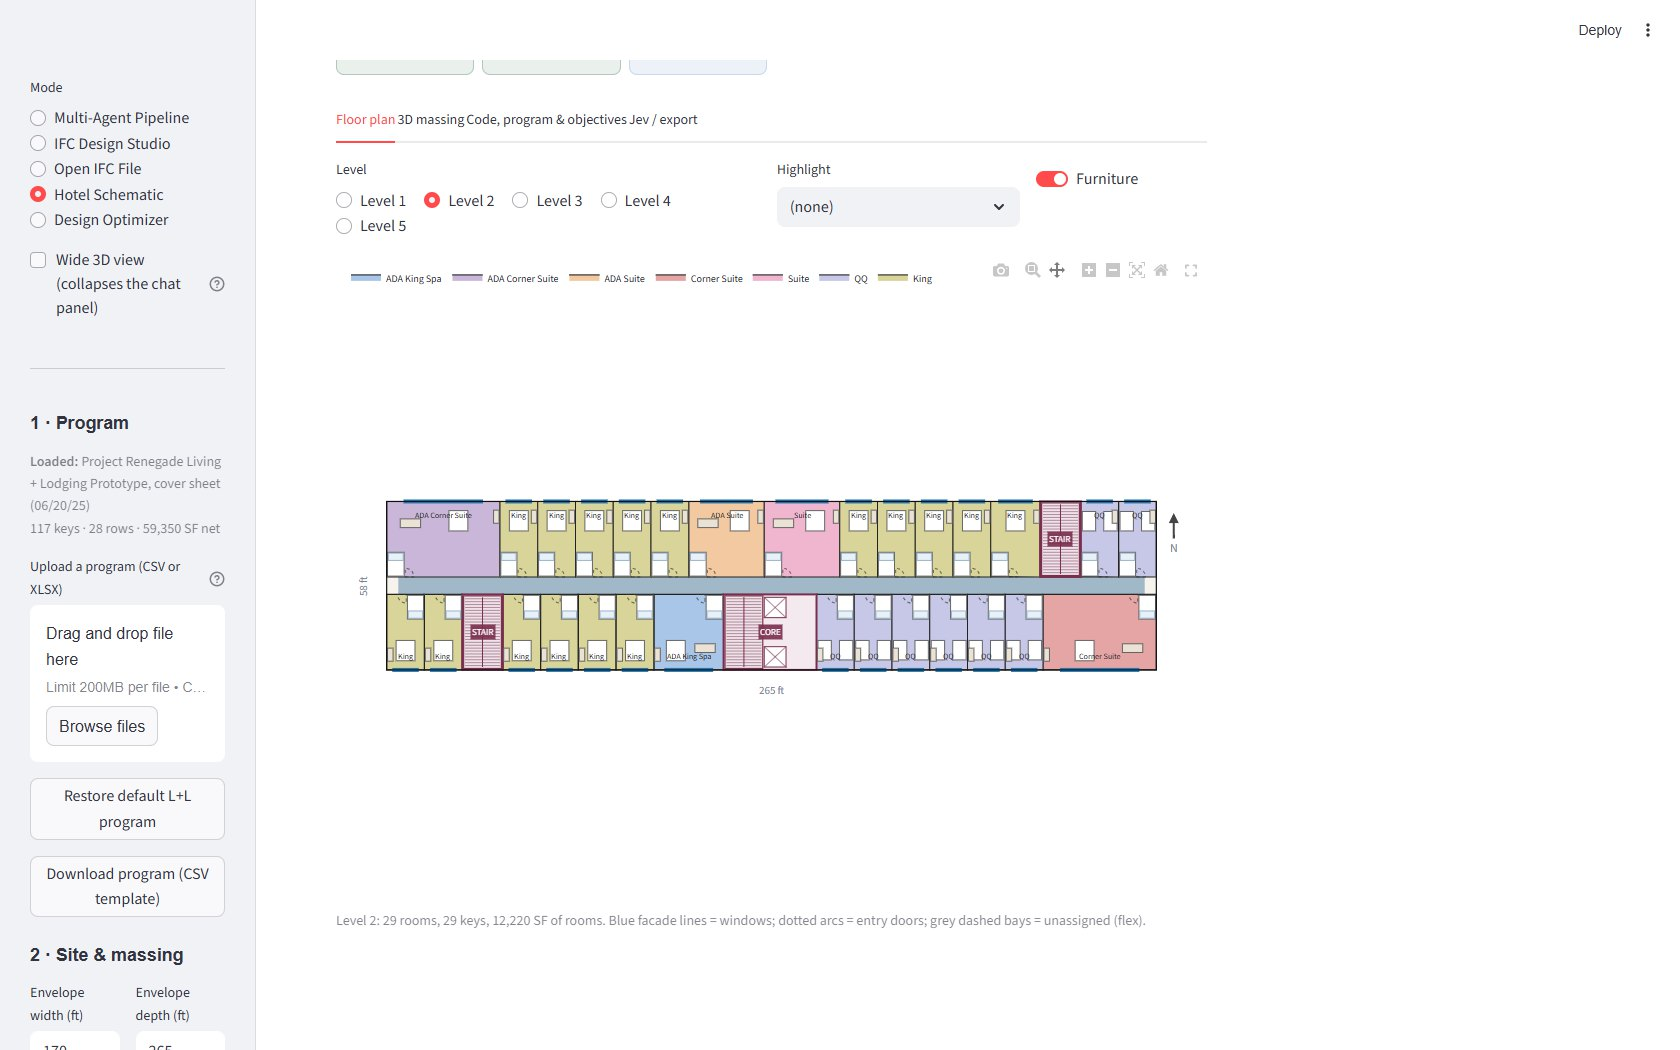
\includegraphics[width=\linewidth,keepaspectratio,height=0.42\textheight]{figures/snap_36_hotel_optimize_plan.jpg}\caption{Interactive furnished plan of the selected layout (hover gives room data).}\end{figure}
\begin{figure}[H]\centering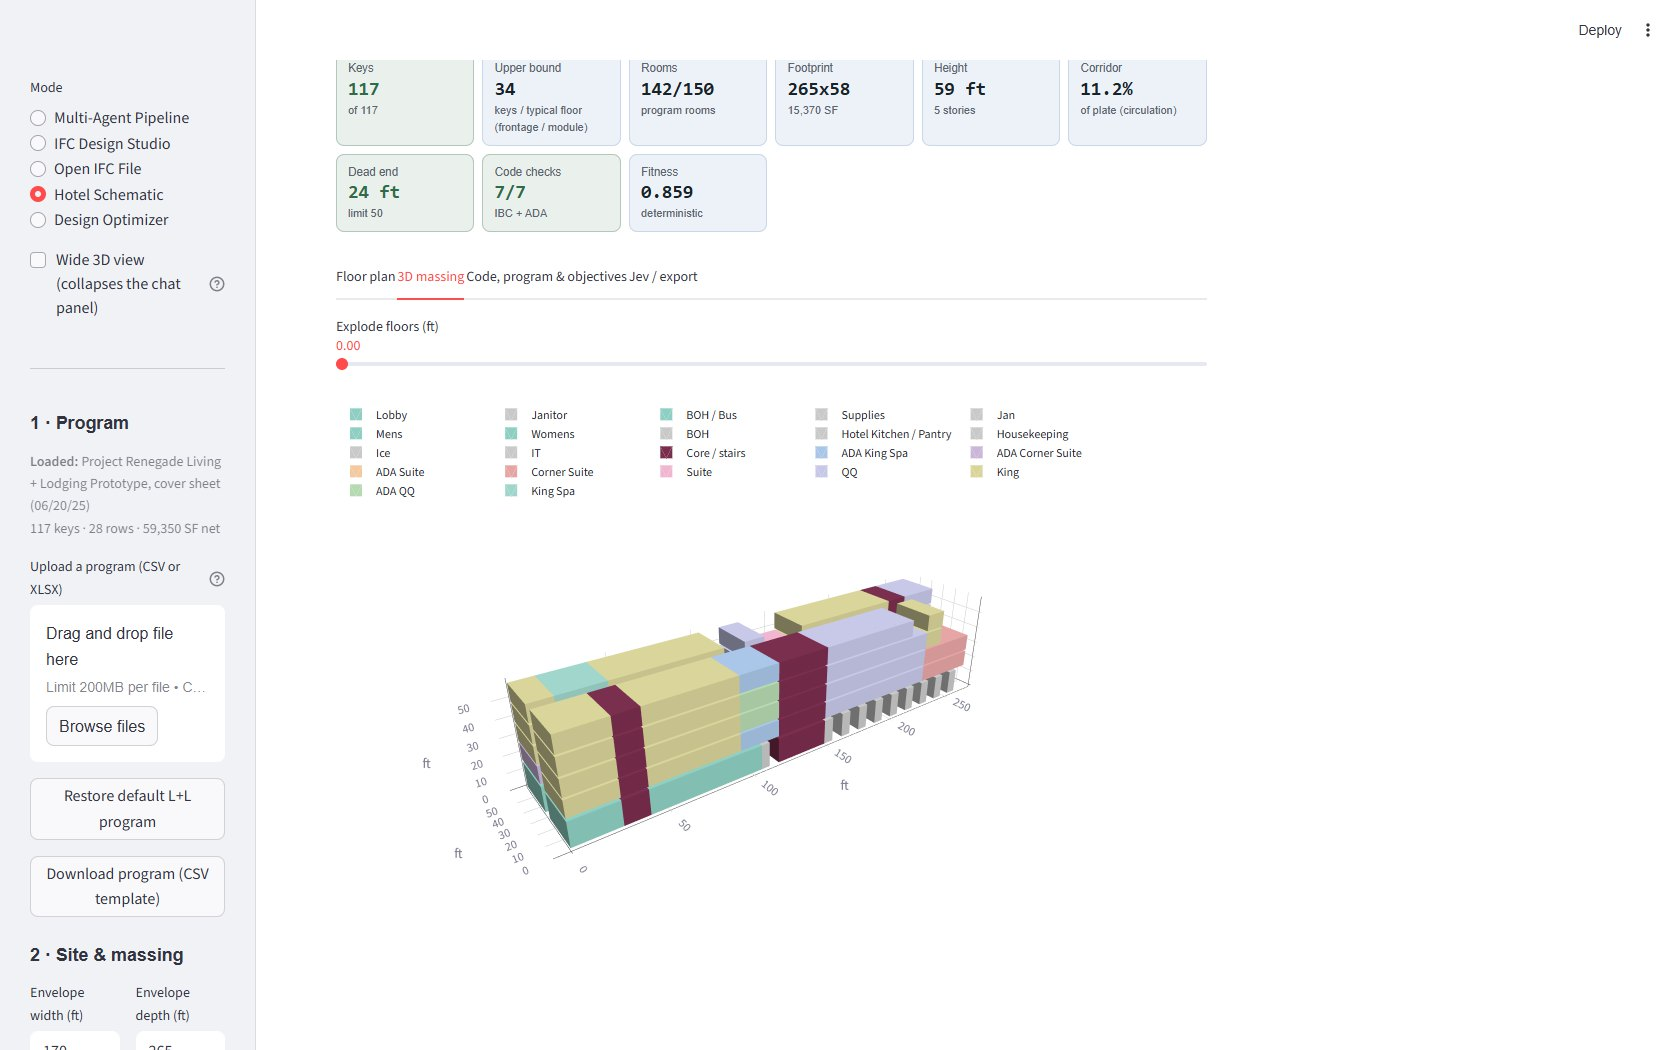
\includegraphics[width=\linewidth,keepaspectratio,height=0.42\textheight]{figures/snap_37_hotel_optimize_3d.jpg}\caption{Stacked 3D massing of the selected layout, coloured by room type.}\end{figure}

\subsection{What is still open}
\begin{itemize}
\item Level 1 uses the same plate as the guest floors (no wider podium), so large ground-floor rooms can be left out; they are listed for every layout.
\item The decoder draws rectangles on a 1 ft grid: angled wings, curved facades and structural grids are not modelled.
\item The upper bounds are loose; a tight bound would need an exact packing model.
\item The centre-core scheme uses two stairs; on T, U and H plates the third wing can exceed the dead-end limit. The check flags it and the ranking moves such layouts down.
\item Parking, cost and energy are not in the fitness. Facade length per key and gross area per key stand in for cost in the decision step.
\item Jev (TypeSafe's hosted decision model) is wired only as an optional advisor; no key was configured for this run.
\end{itemize}
